% -*- Mode:TeX -*-

%% IMPORTANT: The official thesis specifications are available at:
%%            http://libraries.mit.edu/archives/thesis-specs/
%%
%%            Please verify your thesis' formatting and copyright
%%            assignment before submission.  If you notice any
%%            discrepancies between these templates and the 
%%            MIT Libraries' specs, please let us know
%%            by e-mailing thesis@mit.edu

%% The documentclass options along with the pagestyle can be used to generate
%% a technical report, a draft copy, or a regular thesis.  You may need to
%% re-specify the pagestyle after you \include  cover.tex.  For more
%% information, see the first few lines of mitthesis.cls. 

%\documentclass[12pt,vi,twoside]{mitthesis}
%%
%%  If you want your thesis copyright to you instead of MIT, use the
%%  ``vi'' option, as above.
%%
%\documentclass[12pt,twoside,leftblank]{mitthesis}
%%
%% If you want blank pages before new chapters to be labelled ``This
%% Page Intentionally Left Blank'', use the ``leftblank'' option, as
%% above. 

\documentclass[12pt,twoside]{mitthesis}
\usepackage[spanish,es-tabla,es-noquoting]{babel} % Idioma y codificación del texto
\usepackage[utf8x]{inputenc} % Codificación del archivo
\usepackage{hyperref}
\hypersetup{%
    colorlinks=true
}
\usepackage{tikz}
\usepackage{pgfplots}
\pgfplotsset{%
    /pgf/number format/use comma,
    /pgf/number format/set thousands separator = {},
}
\usepackage[justification=centering]{caption}
\usepackage{framed}
\usepackage{caption}
\usepackage{subcaption}
\usepackage{tabu}
\usepackage{fancyvrb}
\usepackage{listings}
%\usepackage{draftwatermark}
%\SetWatermarkText{DRAFT}
%\SetWatermarkScale{5}
%\SetWatermarkColor[rgb]{0.97,0.97,0.97}


%% La tipografía tiene que soportar tildes, no todas lo hacen %%
\usepackage{courier}    % Courier para tipografía monoespaciada
\usepackage{lmodern}
\usepackage[T1]{fontenc}
 
%% Si se usa hyperref + utf8x para establecer el título, autor, etc... %%
\PrerenderUnicode{á}
\PrerenderUnicode{é}
\PrerenderUnicode{í}
\PrerenderUnicode{ó}
\PrerenderUnicode{ú}
\PrerenderUnicode{ñ}

%% Los listings precisan parámetros especiales, sino puede fallar la generación del PDF %%
\lstset{
    numbers=left,
    captionpos=b,
    basicstyle=\ttfamily\footnotesize,
    extendedchars=true,
    inputencoding=utf8x,
    literate={á}{{\'a}}1
          {é}{{\'e}}1
          {í}{{\'i}}1
          {ó}{{\'o}}1
          {ú}{{\'u}}1
          {ñ}{{\~n}}1
}
\renewcommand{\lstlistingname}{Código}
\renewcommand\lstlistlistingname{Índice de códigos}

\usepackage{lgrind}
%% These have been added at the request of the MIT Libraries, because
%% some PDF conversions mess up the ligatures.  -LB, 1/22/2014
\usepackage{cmap}
\usepackage[T1]{fontenc}

%% Citas con un formato más moderno
\usepackage[square]{natbib}

\pagestyle{plain}

\begin{document}

% -*-latex-*-
% 
% For questions, comments, concerns or complaints:
% thesis@mit.edu
% 
%
% $Log: cover.tex,v $
% Revision 1.8  2008/05/13 15:02:15  jdreed
% Degree month is June, not May.  Added note about prevdegrees.
% Arthur Smith's title updated
%
% Revision 1.7  2001/02/08 18:53:16  boojum
% changed some \newpages to \cleardoublepages
%
% Revision 1.6  1999/10/21 14:49:31  boojum
% changed comment referring to documentstyle
%
% Revision 1.5  1999/10/21 14:39:04  boojum
% *** empty log message ***
%
% Revision 1.4  1997/04/18  17:54:10  othomas
% added page numbers on abstract and cover, and made 1 abstract
% page the default rather than 2.  (anne hunter tells me this
% is the new institute standard.)
%
% Revision 1.4  1997/04/18  17:54:10  othomas
% added page numbers on abstract and cover, and made 1 abstract
% page the default rather than 2.  (anne hunter tells me this
% is the new institute standard.)
%
% Revision 1.3  93/05/17  17:06:29  starflt
% Added acknowledgements section (suggested by tompalka)
% 
% Revision 1.2  92/04/22  13:13:13  epeisach
% Fixes for 1991 course 6 requirements
% Phrase "and to grant others the right to do so" has been added to 
% permission clause
% Second copy of abstract is not counted as separate pages so numbering works
% out
% 
% Revision 1.1  92/04/22  13:08:20  epeisach

% NOTE:
% These templates make an effort to conform to the MIT Thesis specifications,
% however the specifications can change.  We recommend that you verify the
% layout of your title page with your thesis advisor and/or the MIT 
% Libraries before printing your final copy.
\title{An Optimizing Compiler for Low-Level Floating Point Operations}

\author{Lucien William Van Elsen}
% If you wish to list your previous degrees on the cover page, use the 
% previous degrees command:
%       \prevdegrees{A.A., Harvard University (1985)}
% You can use the \\ command to list multiple previous degrees
%       \prevdegrees{B.S., University of California (1978) \\
%                    S.M., Massachusetts Institute of Technology (1981)}
\department{Department of Electrical Engineering and Computer Science}

% If the thesis is for two degrees simultaneously, list them both
% separated by \and like this:
% \degree{Doctor of Philosophy \and Master of Science}
\degree{Bachelor of Science in Computer Science and Engineering}

% As of the 2007-08 academic year, valid degree months are September, 
% February, or June.  The default is June.
\degreemonth{June}
\degreeyear{1990}
\thesisdate{May 18, 1990}

%% By default, the thesis will be copyrighted to MIT.  If you need to copyright
%% the thesis to yourself, just specify the `vi' documentclass option.  If for
%% some reason you want to exactly specify the copyright notice text, you can
%% use the \copyrightnoticetext command.  
%\copyrightnoticetext{\copyright IBM, 1990.  Do not open till Xmas.}

% If there is more than one supervisor, use the \supervisor command
% once for each.
\supervisor{William J. Dally}{Associate Professor}

% This is the department committee chairman, not the thesis committee
% chairman.  You should replace this with your Department's Committee
% Chairman.
\chairman{Arthur C. Smith}{Chairman, Department Committee on Graduate Theses}

% Make the titlepage based on the above information.  If you need
% something special and can't use the standard form, you can specify
% the exact text of the titlepage yourself.  Put it in a titlepage
% environment and leave blank lines where you want vertical space.
% The spaces will be adjusted to fill the entire page.  The dotted
% lines for the signatures are made with the \signature command.
\maketitle

% The abstractpage environment sets up everything on the page except
% the text itself.  The title and other header material are put at the
% top of the page, and the supervisors are listed at the bottom.  A
% new page is begun both before and after.  Of course, an abstract may
% be more than one page itself.  If you need more control over the
% format of the page, you can use the abstract environment, which puts
% the word "Abstract" at the beginning and single spaces its text.

%% You can either \input (*not* \include) your abstract file, or you can put
%% the text of the abstract directly between the \begin{abstractpage} and
%% \end{abstractpage} commands.

% First copy: start a new page, and save the page number.
\cleardoublepage
% Uncomment the next line if you do NOT want a page number on your
% abstract and acknowledgments pages.
% \pagestyle{empty}
\setcounter{savepage}{\thepage}
\begin{abstractpage}
% $Log: abstract.tex,v $
% Revision 1.1  93/05/14  14:56:25  starflt
% Initial revision
% 
% Revision 1.1  90/05/04  10:41:01  lwvanels
% Initial revision
% 
%
%% The text of your abstract and nothing else (other than comments) goes here.
%% It will be single-spaced and the rest of the text that is supposed to go on
%% the abstract page will be generated by the abstractpage environment.  This
%% file should be \input (not \include 'd) from cover.tex.
En esta tesina diseñé e implementé un servidor y varios clientes que permiten
programar robots didácticos de forma remota compartiendo un único enlace
físico entre el servidor y los robots y visualizar los movimientos de los
mismos también de forma remota. El servidor implementa un protocolo de capa
de aplicación en base a objetos JSON a través de una conexión WebSocket que
permite a los clientes interactuar con distintos modelos de robots con gran
flexibilidad, moverlos y acceder a los valores de sus sensores, además de
facilitar la visualización de los mismos a través de streaming de video.
Implementé clientes en Javascript (a ser usado desde el navegador),
Python y Ruby que permiten que este proyecto sea utilizado para enseñar
cualquiera de estos lenguajes de programación, además de diseñar y documentar
el protocolo de capa de aplicación para que sea relativamente sencillo
implementar otros clientes.


\end{abstractpage}

% Additional copy: start a new page, and reset the page number.  This way,
% the second copy of the abstract is not counted as separate pages.
% Uncomment the next 6 lines if you need two copies of the abstract
% page.
% \setcounter{page}{\thesavepage}
% \begin{abstractpage}
% % $Log: abstract.tex,v $
% Revision 1.1  93/05/14  14:56:25  starflt
% Initial revision
% 
% Revision 1.1  90/05/04  10:41:01  lwvanels
% Initial revision
% 
%
%% The text of your abstract and nothing else (other than comments) goes here.
%% It will be single-spaced and the rest of the text that is supposed to go on
%% the abstract page will be generated by the abstractpage environment.  This
%% file should be \input (not \include 'd) from cover.tex.
En esta tesina diseñé e implementé un servidor y varios clientes que permiten
programar robots didácticos de forma remota compartiendo un único enlace
físico entre el servidor y los robots y visualizar los movimientos de los
mismos también de forma remota. El servidor implementa un protocolo de capa
de aplicación en base a objetos JSON a través de una conexión WebSocket que
permite a los clientes interactuar con distintos modelos de robots con gran
flexibilidad, moverlos y acceder a los valores de sus sensores, además de
facilitar la visualización de los mismos a través de streaming de video.
Implementé clientes en Javascript (a ser usado desde el navegador),
Python y Ruby que permiten que este proyecto sea utilizado para enseñar
cualquiera de estos lenguajes de programación, además de diseñar y documentar
el protocolo de capa de aplicación para que sea relativamente sencillo
implementar otros clientes.


% \end{abstractpage}

\cleardoublepage

\section*{Acknowledgments}

This is the acknowledgements section.  You should replace this with your
own acknowledgements.

%%%%%%%%%%%%%%%%%%%%%%%%%%%%%%%%%%%%%%%%%%%%%%%%%%%%%%%%%%%%%%%%%%%%%%
% -*-latex-*-

% Some departments (e.g. 5) require an additional signature page.  See
% signature.tex for more information and uncomment the following line if
% applicable.
% % -*- Mode:TeX -*-
%
% Some departments (e.g. Chemistry) require an additional cover page
% with signatures of the thesis committee.  Please check with your
% thesis advisor or other appropriate person to determine if such a 
% page is required for your thesis.  
%
% If you choose not to use the "titlepage" environment, a \newpage
% commands, and several \vspace{\fill} commands may be necessary to
% achieve the required spacing.  The \signature command is defined in
% the "mitthesis" class
%
% The following sample appears courtesy of Ben Kaduk <kaduk@mit.edu> and
% was used in his June 2012 doctoral thesis in Chemistry. 

\begin{titlepage}
\begin{large}
This doctoral thesis has been examined by a Committee of the Department
of Chemistry as follows:

\signature{Professor Jianshu Cao}{Chairman, Thesis Committee \\
   Professor of Chemistry}

\signature{Professor Troy Van Voorhis}{Thesis Supervisor \\
   Associate Professor of Chemistry}

\signature{Professor Robert W. Field}{Member, Thesis Committee \\
   Haslam and Dewey Professor of Chemistry}
\end{large}
\end{titlepage}


\pagestyle{plain}
  % -*- Mode:TeX -*-
%% This file simply contains the commands that actually generate the table of
%% contents and lists of figures and tables.  You can omit any or all of
%% these files by simply taking out the appropriate command.  For more
%% information on these files, see appendix C.3.3 of the LaTeX manual. 
\tableofcontents
\newpage
\listoffigures
\newpage
\lstlistoflistings
\listoftables


\chapter*{Prólogo}\label{cha:prologo}


Esta tesina se enmarca en el proyecto \proyecto{} del
LINTI\footnote{\url{http://linti.unlp.edu.ar}}
y el desarrollo realizado
es una contribución a dicho proyecto.
Se implementó un servidor denominado XRemoteBot y tres
clientes compatibles
con el mismo escritos en tres lenguajes distintos. El motivo y las elecciones hechas
en el desarrollo del servidor y los clientes serán relatados a lo largo de este
trabajo.

A continuación se describe la forma en que se ha organizado este informe y en el CD
adjunto se entrega tanto una copia del mismo como los fuentes desarrollados.
Aunque
cabe aclarar que todo el trabajo implementado ha sido desarrollado con software libre,
será liberado bajo licencia
MIT\footnote{\url{http://opensource.org/licenses/MIT}} y se puede descargar
desde GitHub\footnote{%
\url{https://github.com/fernandolopez/xremotebot} y
\url{https://github.com/fernandolopez/xremotebot-clients}}.

El capítulo~\ref{cha:motivacion} relata la motivación para el desarrollo de
XRemoteBot.

El capítulo~\ref{cha:arte} presenta un relevamiento de desarrollos y
proyectos similares.

El capítulo~\ref{cha:myro_y_duinobot} describe el modo funcionamiento de las
bibliotecas usadas hasta el momento en el proyecto \proyecto{} para
interactuar con los robots, estas
bibliotecas son la base de XRemoteBot.

El capítulo~\ref{cha:xremotebot} describe el modo de funcionamiento y
tecnologías utilizadas en el servidor
XRemoteBot desarrollado para esta tesina y de su antecesor RemoteBot.

El capítulo~\ref{cha:clientes} describe el modo de uso, modo de
funcionamiento y
tecnologías utilizadas en los tres clientes desarrollados para
XRemoteBot, especialmente el cliente Javascript que es el más complejo
en su implementación.

El capítulo~\ref{cha:protocolo} describe el protocolo de capa de aplicación diseñado para
el servidor desarrollado y las modalidades de operación del mismo.

El capítulo~\ref{cha:pruebas} describe el entorno en el que fue probado
XRemoteBot, detallando algunas de pruebas realizadas y algunas
modificaciones
realizadas al proyecto en base a los resultados de estas pruebas.

El capítulo~\ref{cha:conclusiones} contiene las conclusiones del trabajo
y el trabajo a futuro.

%% This is an example first chapter.  You should put chapter/appendix that you
%% write into a separate file, and add a line \include{yourfilename} to
%% main.tex, where `yourfilename.tex' is the name of the chapter/appendix file.
%% You can process specific files by typing their names in at the 
%% \files=
%% prompt when you run the file main.tex through LaTeX.
\chapter{Motivación del diseño y desarrollo de XRemoteBot}\label{cha:motivacion}

En este capítulo se describen los motivos que llevaron a implementar XRemoteBot
como
parte de esta tesina, como así también las decisiones
iniciales de
diseño y la decisión del lenguaje de programación en el cuál se implementará
la mayor
parte de la aplicación.


\section{Motivación}\label{sec:motivacion}
Desde el año 2009, en el marco del proyecto ``Programando con robots y
software libre'' del LINTI\footnote{\url{http://robots.linti.unlp.edu.ar}},
se utilizan robots para enseñar programación en Python a alumnos de escuelas
secundarias. Estos robots son la herramienta didáctica que permite enseñar
las estructuras básicas del lenguaje Python.

\begin{figure}
    \centering
    \begin{subfigure}[b]{0.49\textwidth}
        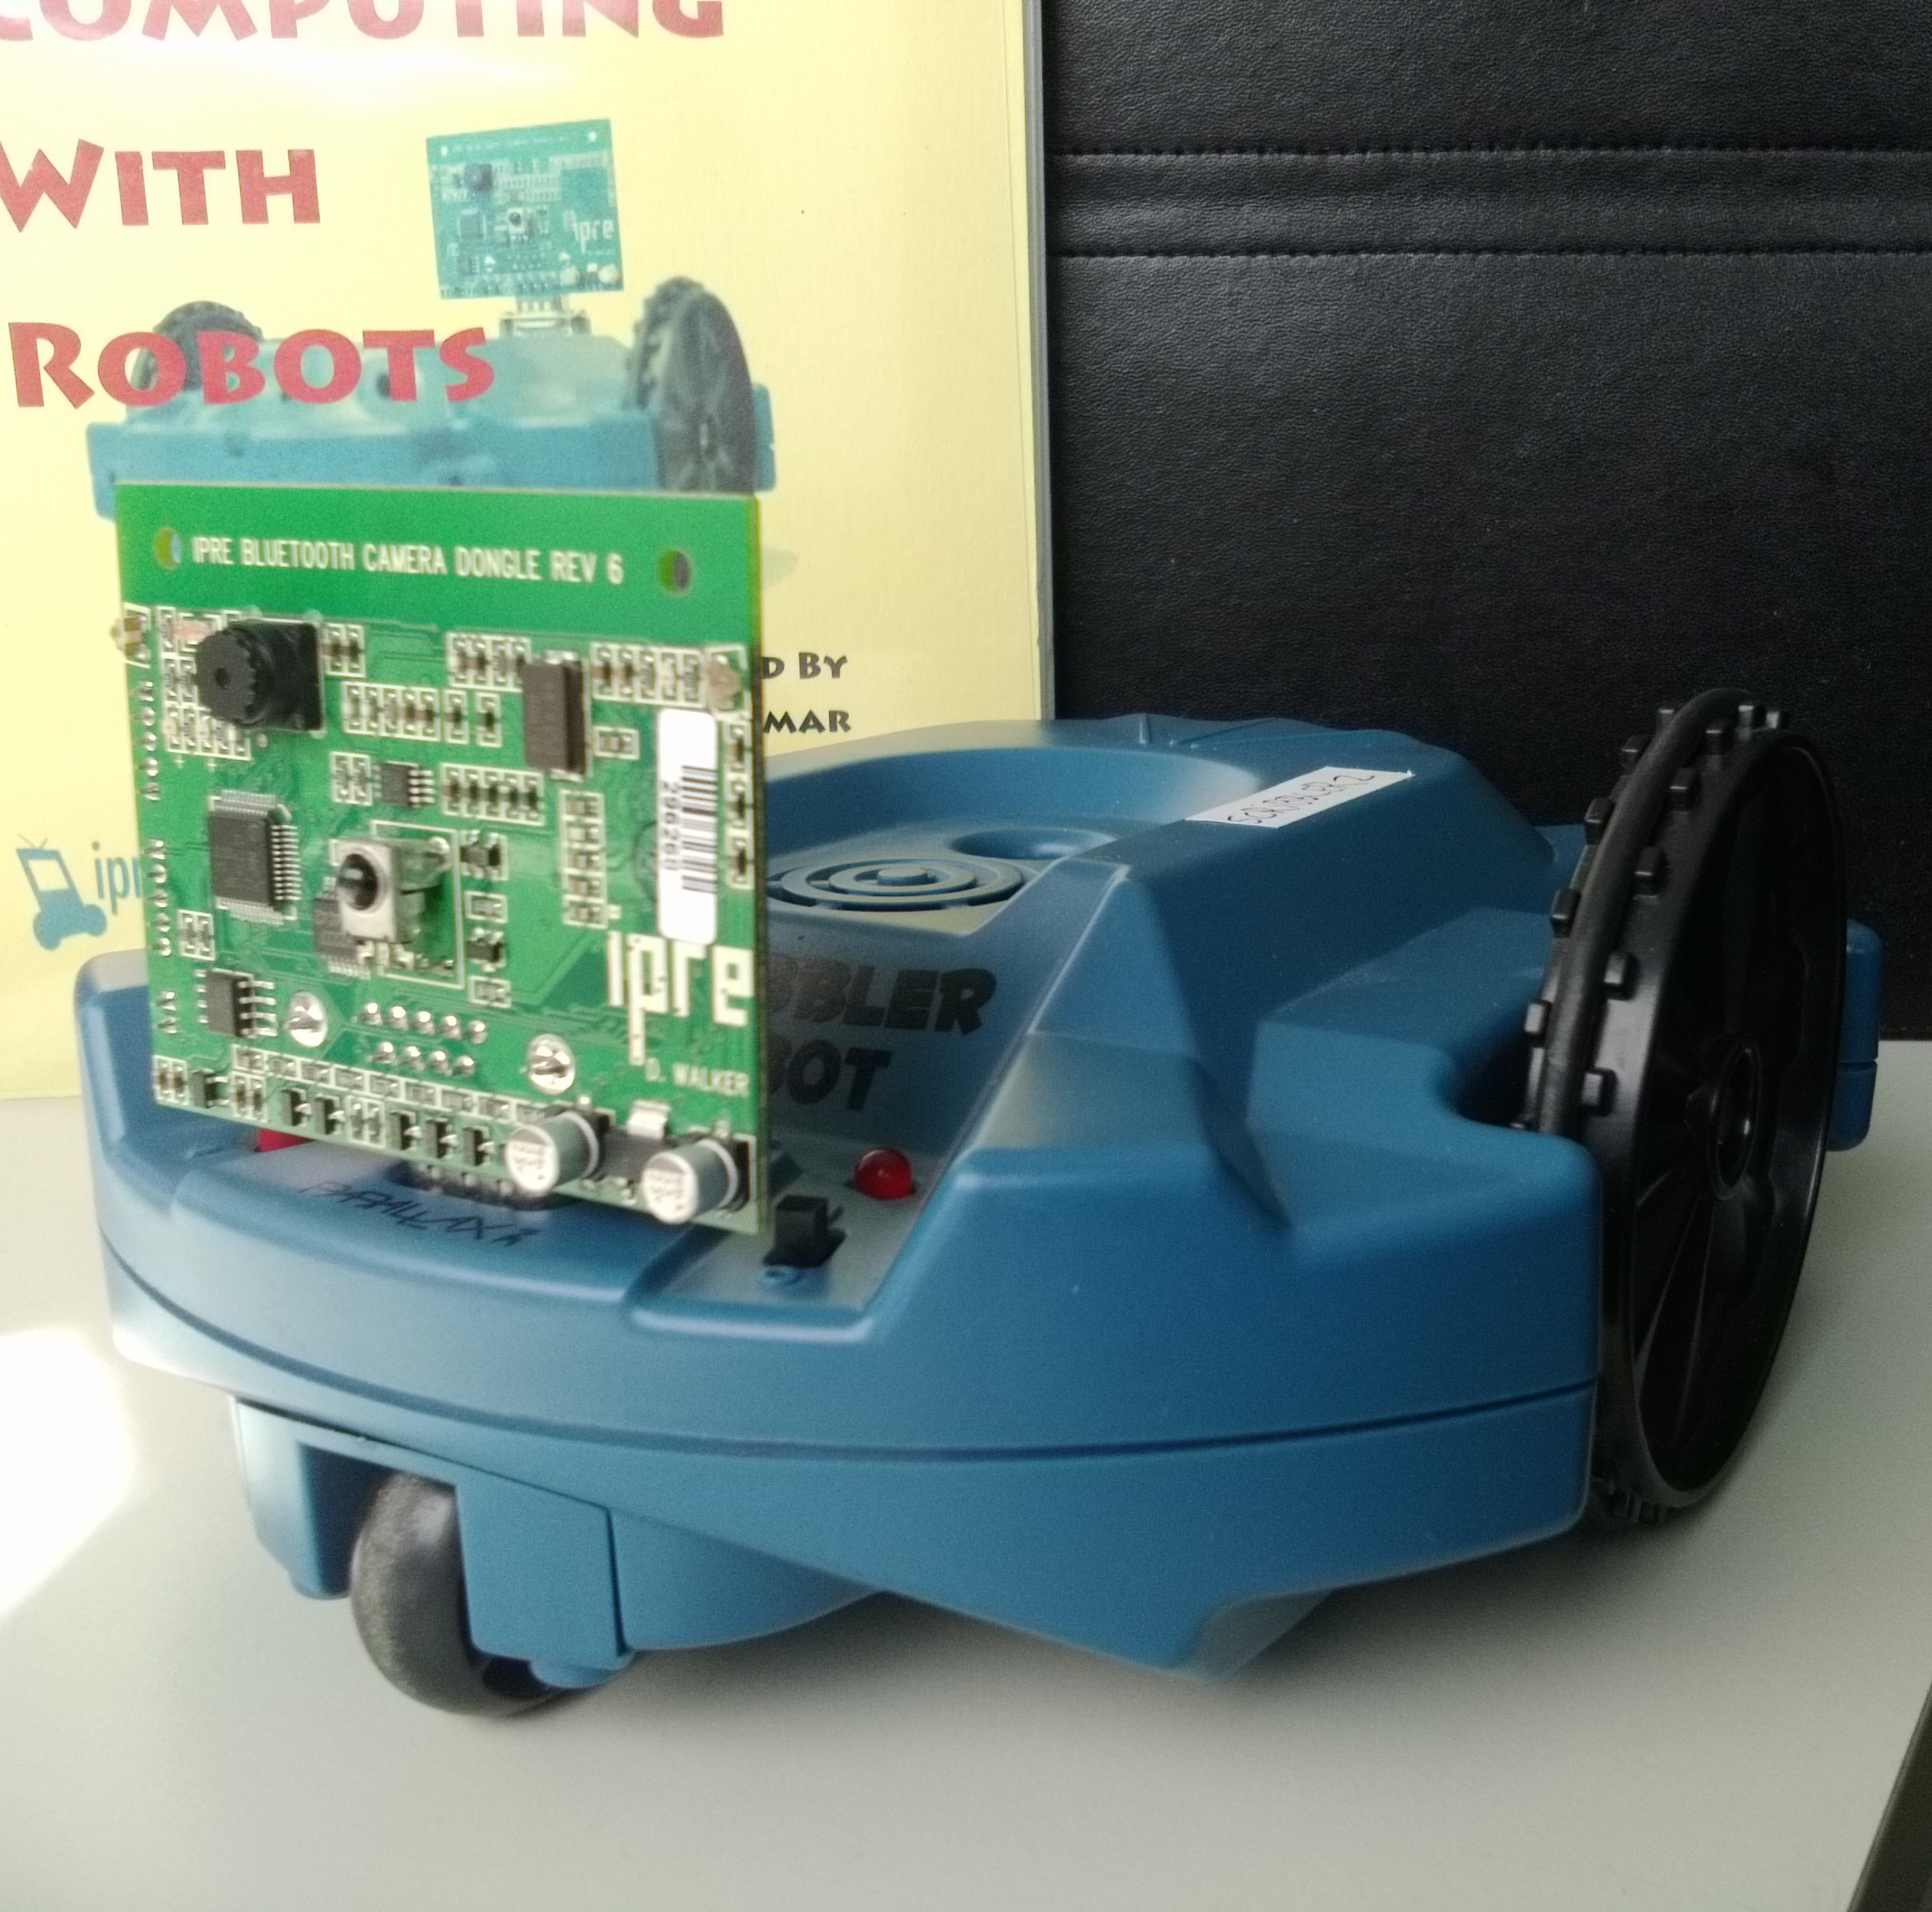
\includegraphics[width=\textwidth]{figures/scribbler}
        \subcaption{Robot Scribbler de Parallax}\label{fig:robots_usados_scribbler}
    \end{subfigure}
    \begin{subfigure}[b]{0.49\textwidth}
        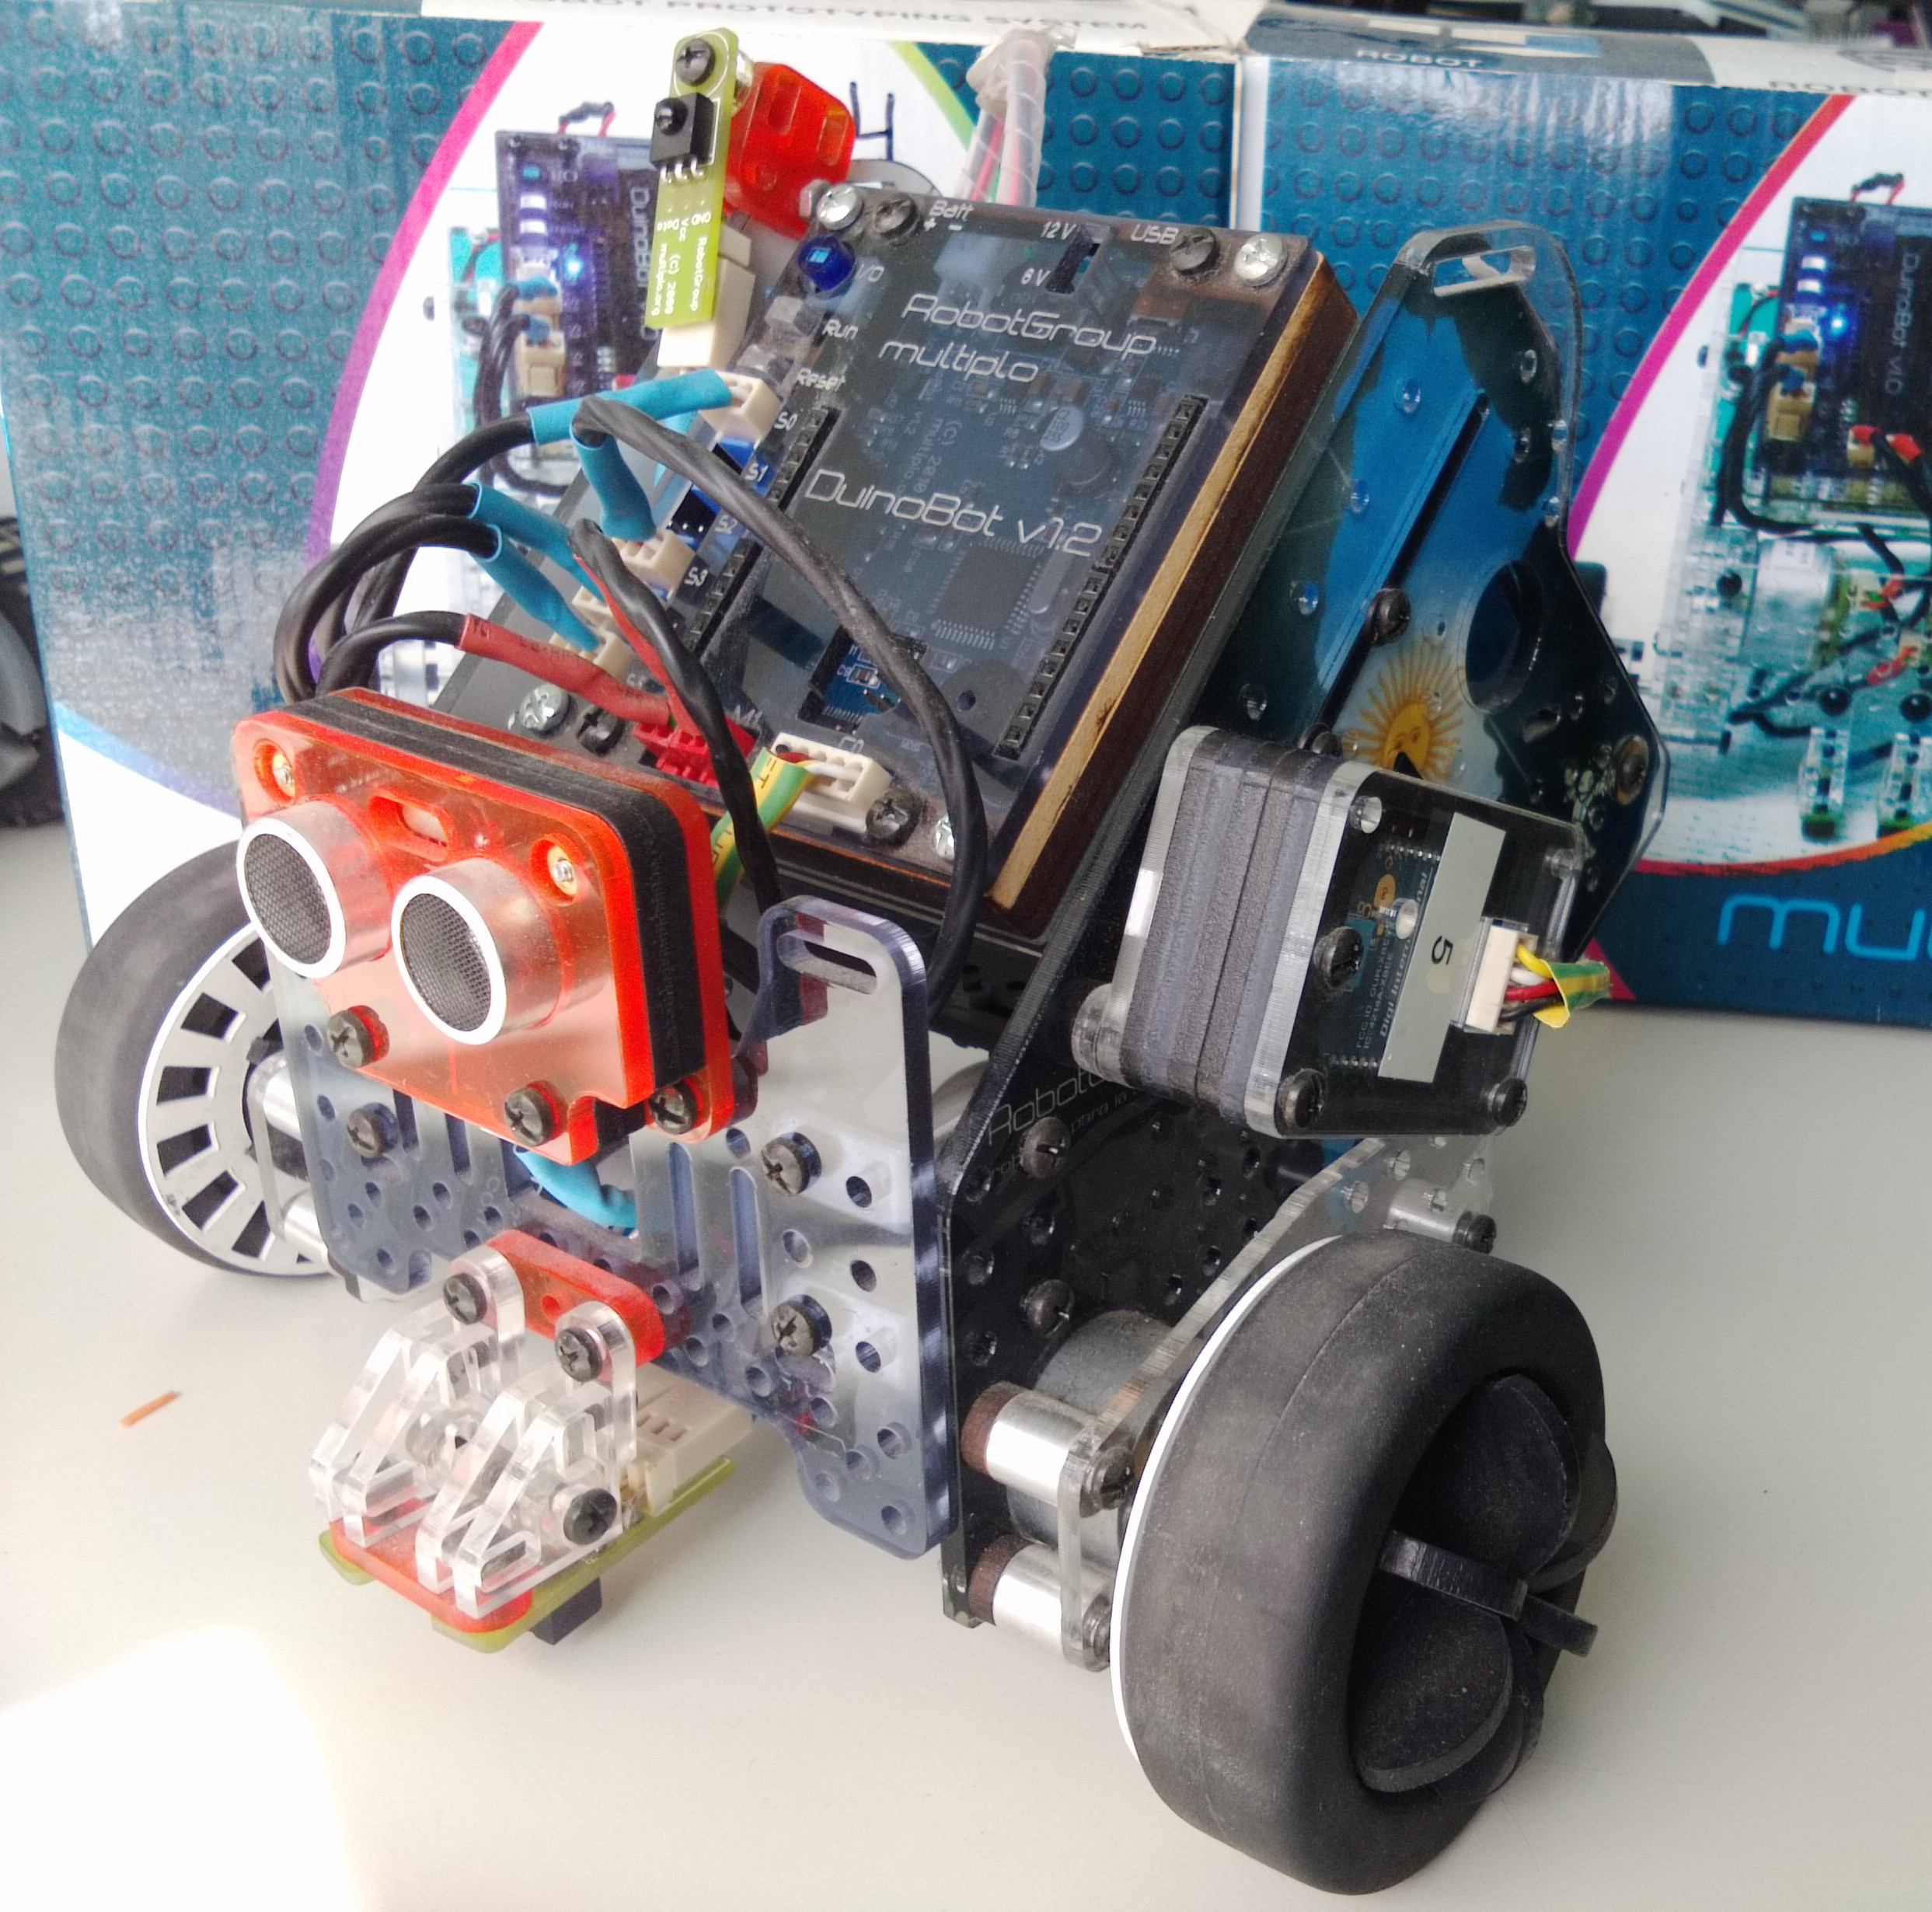
\includegraphics[width=\textwidth]{figures/n6}
        \subcaption{Robot Multiplo N6 de RobotGroup}\label{fig:robots_usados_n6}
    \end{subfigure}
    \caption{Robots usados en el proyecto}\label{fig:robots_usados}
\end{figure}

En un comienzo se utilizaron los robots Scribbler de Parallax, mostrados en
la figura~\ref{fig:robots_usados_scribbler}. Estos robots pueden programarse
directamente a través de un cable utilizando el lenguaje
PBASIC\footnote{\url{http://homepages.ius.edu/RWISMAN/C490/html/PythonandRobots.htm}
y\\ \url{http://learn.parallax.com/teach/pbasic-programming-basic-stamp}}
y funcionar de forma autónoma, o pueden ser controlados de forma
inalámbrica incorporando un dispositivo extra y conectándose por Bluetooth.

En las experiencias realizadas se los utilizó de
la última
forma, y de esta manera se controla el robot usando el lenguaje Python
(cuyo intérprete no
es posible ejecutar directamente sobre el microcontrolador del mismo).

Los robots Scribbler se importan desde Estados Unidos en volúmenes bajos
por las restricciones a la importación en nuestro país, lo que
dificulta su adquisición tanto por el equipo del proyecto como de posibles
escuelas que quisieran comprarlos, dejando, además al equipo sin ninguna
garantía
ante posibles averías. Por estos motivos, se buscaron alternativas de
fabricación nacional,
que pudieran ser programados en lenguaje Python y tuvieran especificaciones
abiertas.
De esta manera, a fines del año 2011, se adquirieron dos robots Multiplo N6
de fabricación nacional de
la empresa RobotGroup, mostrados en la figura~\ref{fig:robots_usados_n6}.
Tanto el software necesario para controlar estos robots como sus
especificaciones se distribuyen bajo una licencia
abierta\footnote{\url{https://www.kickstarter.com/projects/1689254125/multiplo-create-your-own-robot/description}}.

Los robots Multiplo N6 están basados en
Arduino\footnote{\url{http://www.arduino.cc/}}
por lo que pueden ser programados
usando el IDE Arduino en C++. Además RobotGroup ofrece el entorno de programación
MiniBloq que permite programar el robot de forma gráfica usando bloques.
Dado que estas modalidades no se adecuaban a las propuestas del proyecto
se pidió a la empresa una versión modificada del robot para controlarlo de forma
inalámbrica (ya que no es posible ejecutar un intérprete CPython en una
placa de esas características) y se
desarrolló
una biblioteca Python que permite la programación del robot en dicho lenguaje. Este
desarrollo fue realizado en forma conjunta entre el equipo del proyecto \proyecto{}
y miembros de la empresa RobotGroup, y actualmente está
siendo mantenido por el LINTI~\citep{diaz_aprendiendo_2012}.

La biblioteca Python que permite controlar los robots Multiplo N6 se
denomina DuinoBot. Se eligió este nombre por coincidir con el de la placa
controladora de los robots, sin embargo en este informe DuinoBot hace
referencia a la biblioteca Python desarrollada en conjunto
entre el equipo del proyecto \proyecto{} y la empresa RobotGroup.

En el año 2012, a través de un convenio de cooperación con la Fundación YPF,
que brindó
un subsidio, y bajo el auspicio de la Dirección de Escuelas Técnicas de la
Provincia de Buenos Aires se realizó una
capacitación en 10 escuelas técnicas de la
provincia de Buenos Aires. La Fundación YPF brindó a cada una de estas
escuelas, entre otras
cosas, 20 robots Multiplo N6 que quedaron en cada escuela. En estos cursos
se capacitaron más de 140 docentes y 40 alumnos avanzados, en programación
en el lenguaje Python utilizando
estos dispositivos~\citep{diaz_aprendiendo_2012} como herramienta didáctica.

Esta experiencia consolidó el uso de
los robots Multiplo N6 en el proyecto
``Programando con robots y software libre'', reemplazando
a los robots Scribblers, tanto por su confiabilidad como por su facilidad de
adquisición.

\section{Los robots}
Como se mencionó anteriormente, se utilizaron a lo largo del proyecto dos
modelos de robots distintos: el Scribbler y el Multiplo N6. Esta sección provee una
breve descripción de sus características técnicas.

\subsection{Robot Scribbler de Parallax}
Los robots Scribbler (versión 1) cuentan con un microcontrolador
\textit{PIC16F57}\footnote{Esta información se obtuvo con una inspección
visual de uno de estos robots.}
que viene programado con un intérprete de Basic. El producto
completo es denominado por Parallax
``Basic Stamp 2''\footnote{\url{http://www.andybrain.com/extras/scribbler-robot-review.htm}}.
Para su locomoción este robot cuenta con dos ruedas conectadas a través de
cajas
reductoras
a sus respectivos motores de DC (corriente continua)  y una tercer rueda no conectada a ningún
motor que sirve como tercer punto de apoyo para el cuerpo del robot.

La alimentación eléctrica del robot es provista por 6 pilas AA.

En cuanto a los sensores, este robot está equipado con:
\begin{itemize}
    \item Dos emisores infrarrojos a los lados de su parte frontal y un
        sensor infrarrojo entre ellos que permite sensar (de acuerdo a si se
        refleja el haz de luz infrarroja de alguno de los laterales) si
        hay algún obstáculo a la derecha o a la izquierda del robot.
    \item Tres fotorresistores ubicados dentro de 3 cavidades al frente del
        robot que permiten sensar la presencia de fuentes de luz e
        identificar (si la luz no es muy difusa) si las mismas se encuentran
        directamente enfrente, a la izquierda o a la derecha del robot.
    \item Dos sensores de línea que consisten cada uno de un emisor
        y un sensor infrarrojo (IR). Los mismos detectan cambios de contraste
        en el piso de acuerdo a la cantidad de luz IR reflejada y generalmente
        se utilizan para que el robot siga un camino demarcado por una línea
        de un color sobre una superficie de un color contrastante.
\end{itemize}

\begin{figure}
    \centering
    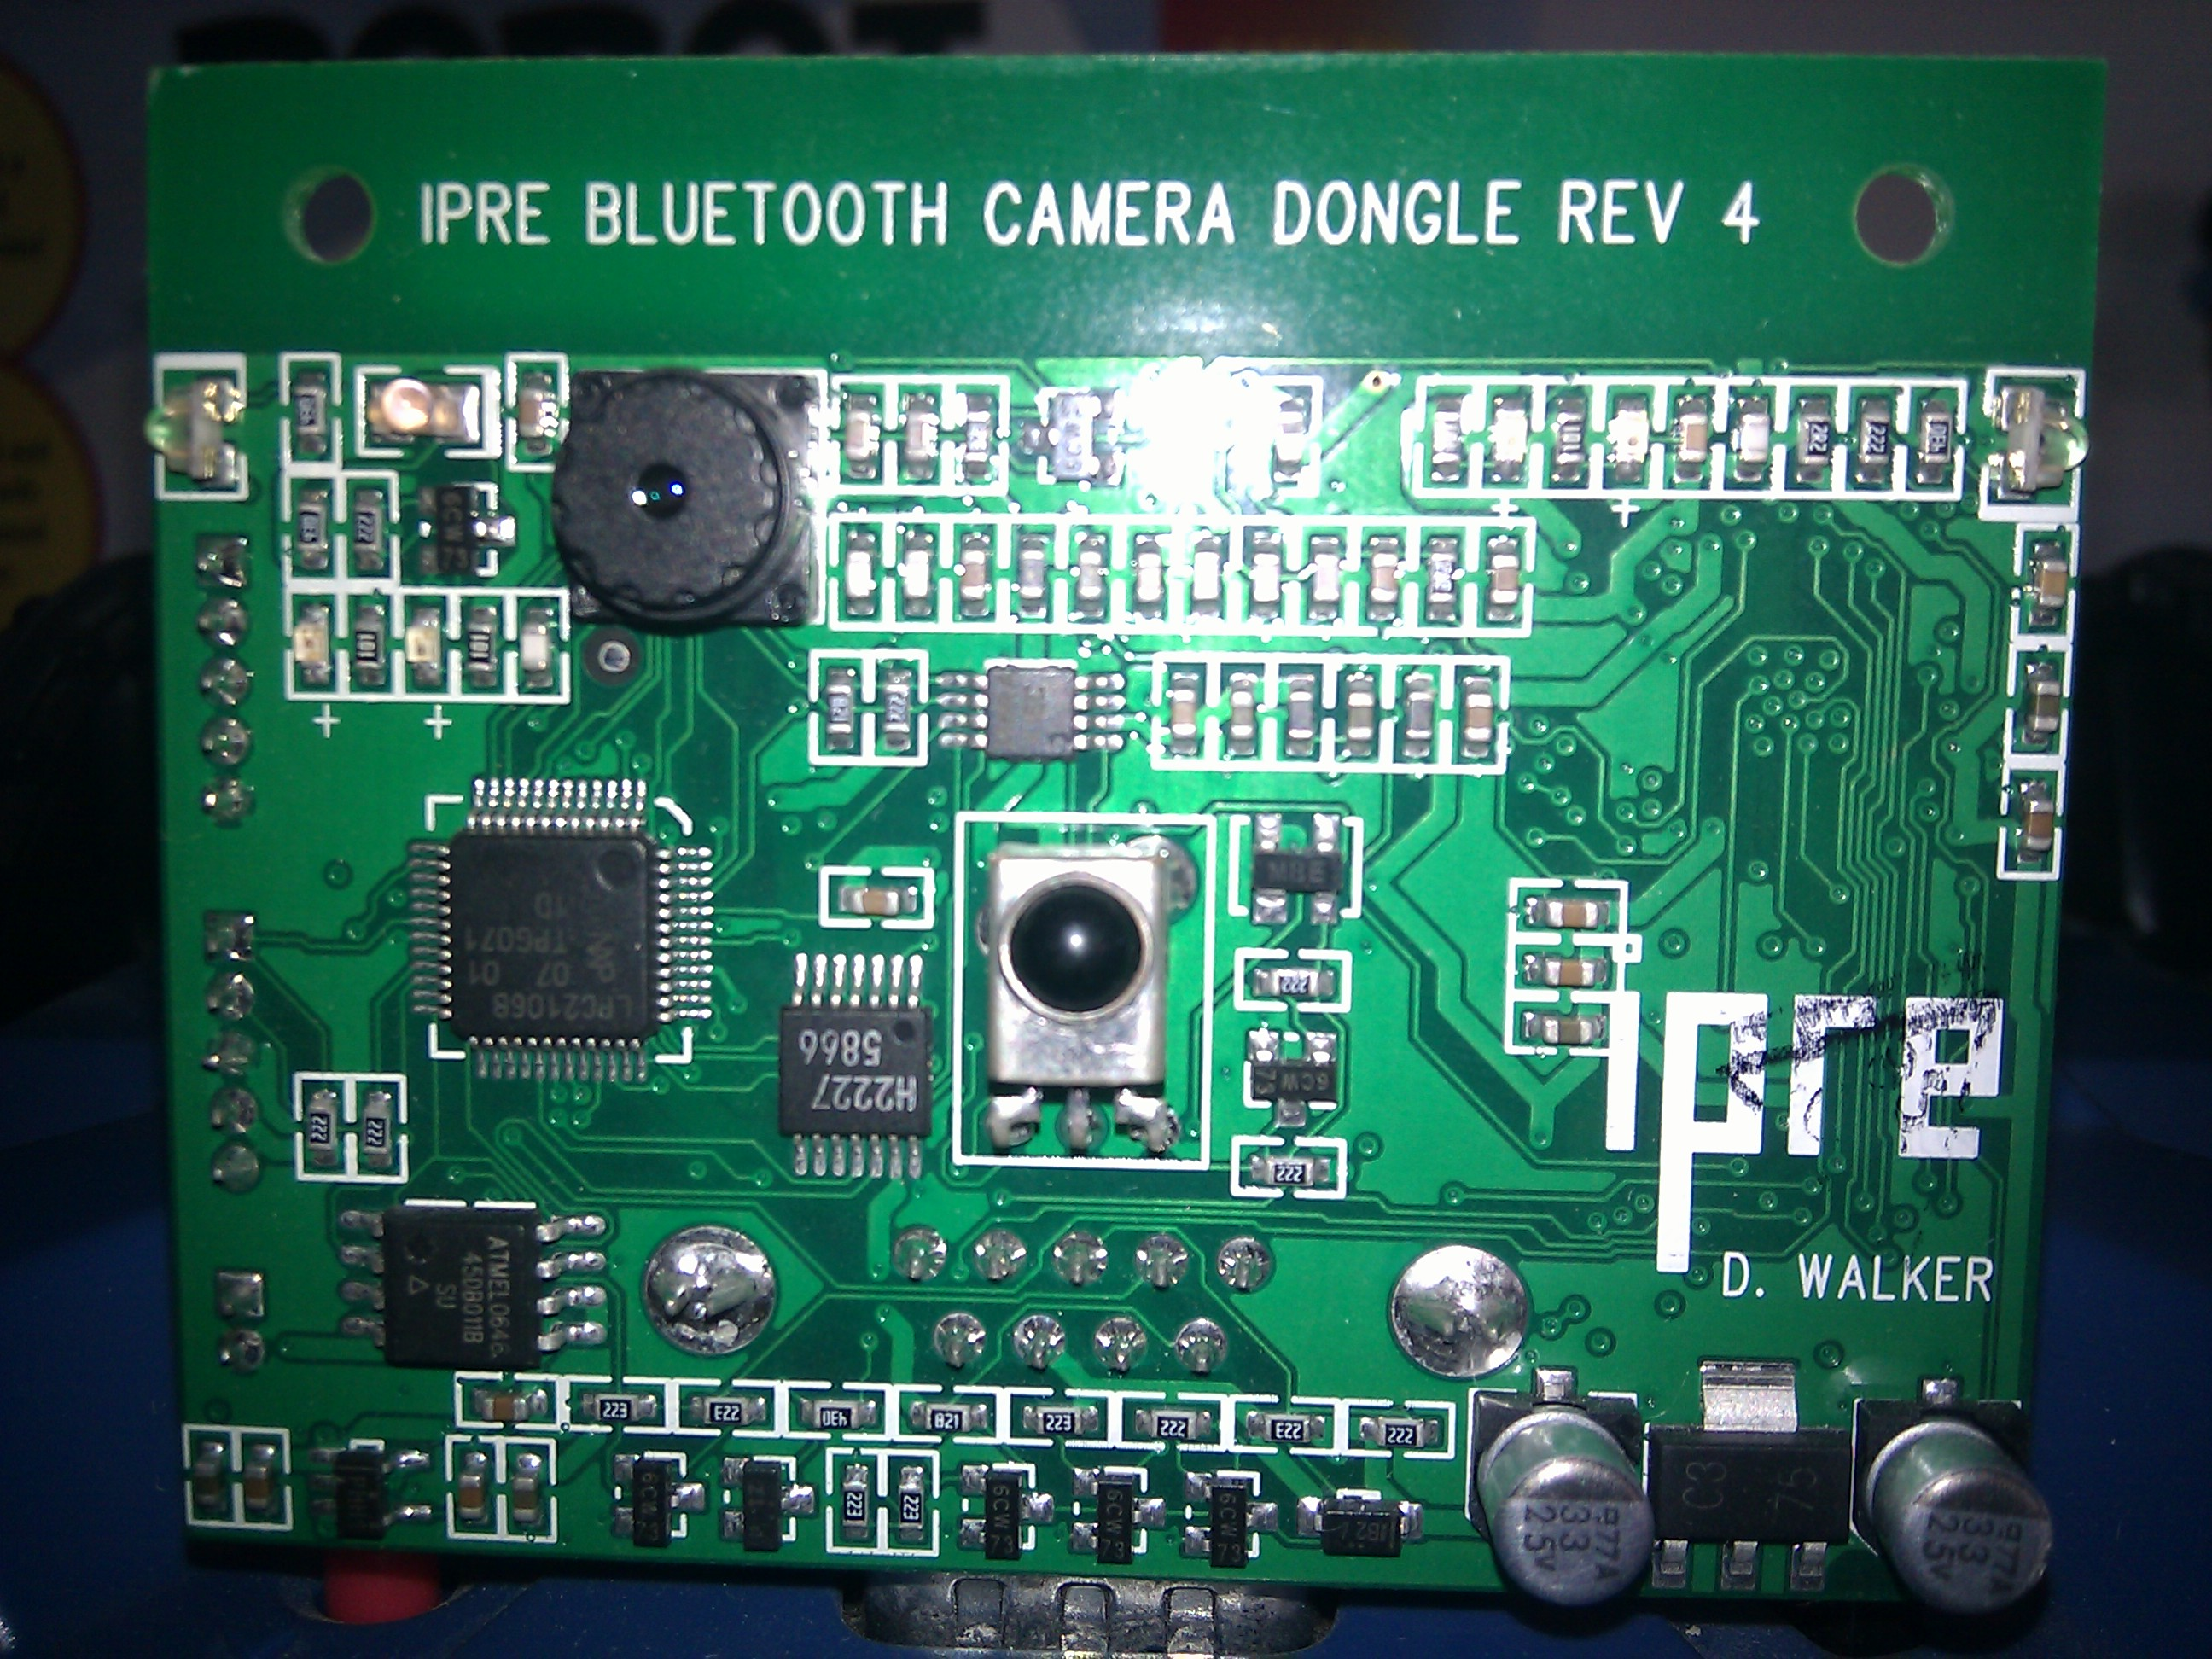
\includegraphics[width=0.5\linewidth]{figures/fluke}
    \caption{IPRE Fluke}
    \label{fig:foto_fluke}
\end{figure}

Si bien las anteriores son las características generales de estos robots, usándolos
de esta manera es necesario programarlos a través de un cable serial usando el
lenguaje PBASIC basado en BASIC. Para las actividades planteadas en el marco del
proyecto \proyecto{}, se utilizó  una versión
que agrega un dispositivo extra: el IPRE Fluke~\ref{fig:foto_fluke}.
Este dispositivo se conecta al puerto
serial del robot y provee la capacidad de controlarlo de forma inalámbrica
usando Bluetooth.  Conectar el
IPRE Fluke invierte el sentido de giro de las ruedas, por lo que el frente
del robot pasa a ser el lugar donde se conecta el IPRE Fluke. De aquí
en adelante cuando se mencione la parte delantera del Scribbler, será la
parte donde se encuentra conectado el IPRE Fluke y la parte trasera será la
opuesta.

El IPRE Fluke es comandado por con un microcontrolador
\textit{LPC2106F}\footnote{Información obtenida con una inspección visual
de la placa.}
basado en la arquitectura
\textit{ARM7}\footnote{\url{http://pdf1.alldatasheet.com/datasheet-pdf/view/83950/PHILIPS/LPC2106FHN48.html}}. Posee un módulo de comunicaciones
Bluetooth que utiliza como medio de comunicación con la computadora
controlante y
provee una cámara de baja resolución con la que se pueden tomar fotografías,
que luego serán transmitidas por Bluetooth. Además agrega
un sensor infrarrojo que permite detectar la presencia de obstáculos
a la izquierda, al centro o a la derecha (está compuesto de 3 emisores
y un
receptor)\footnote{\url{http://wiki.roboteducation.org/Myro_Hardware}}.
Con esta incorporación el robot queda equipado ahora con sensores
en la parte frontal y en la parte trasera, pero más importante aún
el módulo Bluetooth permite controlarlo de forma inalámbrica siempre
que se grabe un firmware especial en la placa IPRE Fluke. Esto es lo que permite
que estos robots puedan ser programados con Python usando una biblioteca denominada
\textit{Myro}\footnote{\url{http://wiki.roboteducation.org/Myro_Reference_Manual}},
que será descripta en la sección~\ref{sec:myro}.

\subsection{Multiplo N6}
El robot Multiplo N6, fabricado por la empresa RobotGroup, cuenta con un
microcontrolador Atmel
\textit{AVR ATMega32U4}\footnote{\url{http://www.robotgroup.com.ar/index.php/productos/131-robot-n6\#especificaciones}}
con el bootloader de Arduino
precargado. Para su locomoción cuenta con dos ruedas conectadas a través
de reductores de velocidad a sus correspondientes motores de
corriente continua y una tercer
rueda no conectada a ningún motor que sirve como tercer punto de apoyo.
La alimentación eléctrica de estos robots está dada por tres pilas AA
en serie (o bien dos packs de tres pilas cada uno en paralelo).

En cuanto a los sensores el Multiplo N6 está equipado con:
\begin{itemize}
    \item Un sensor ultrasónico para detectar obstáculos al frente del
        robot.
    \item Un sensor infrarrojo que puede ser utilizado en conjunto con
        un control remoto universal para enviar comandos al robot
        (siempre que se programe este comportamiento previamente).
    \item Dos sensores detectores de línea, compuestos de un emisor y
        un receptor infrarrojo cada uno. Opcionalmente estos sensores
        pueden desatornillarse y ensamblarse
        para funcionar como
        ``encoders''\footnote{\url{http://machinedesign.com/sensors/basics-rotary-encoders-overview-and-new-technologies-0}}
        de las ruedas y de esta manera es posible
        calcular la velocidad de giro de las ruedas. Este uso
        no es recomendable si se controla el robot de forma remota
        ya que la latencia de las comunicaciones puede hacer que se pierdan
        datos haciendo que el cálculo de la velocidad sea impreciso.
\end{itemize}

En esta configuración estos robots son programables usando el entorno de
Arduino y desde MiniBloq\footnote{\url{http://minibloq.org}}, pero dado que el objetivo del proyecto es la enseñanza de
programación en el lenguaje Python se encargó a la empresa una versión
modificada del Multiplo N6 que permitiera controlarlo de forma inalámbrica,
de manera tal que una computadora con un intérprete de Python instalado
pudiera enviar instrucciones y recibir los valores de los sensores
del robot tal como hace la biblioteca Myro con los robots Scribbler.
Esta
modificación consistió en la adición de un módulo de comunicación inalámbrica
XBee
que permite enviar y recibir datos del robot a través del protocolo
ZigBee\footnote{\url{http://www.digi.com/xbee/}}, la modificación de
un firmware basado en una implementación existente para Arduino del protocolo
de control \texttt{Firmata}\footnote{\url{http://firmata.org/}} y el
desarrollo
del módulo Python \texttt{DuinoBot} para controlar a los robots usando
este protocolo, el
cuál fue adaptado por los miembros del proyecto \proyecto{}
para soportar nuevas funcionalidades y proveer una
API similar a la de la biblioteca
\texttt{Myro}\citep{lanfranco_2012}.

Básicamente los robots Multiplo N6 utilizados en el proyecto \proyecto{}
contienen un
firmware basado en Firmata, modificado para soportar
las características propias del robot. Este firmware recibe instrucciones desde
un un puerto serie conectado a una placa XBee y envía las respuestas
a la misma utilizando una variación del protocolo Firmata. Desde el lado
de la computadora controlante, el módulo DuinoBot provee una interfaz
de alto nivel para los alumnos, donde cada instrucción para el robot
programada
en Python se convierte a una secuencia de bytes del protocolo Firmata
y se envía al robot a través de una placa XBee conectada por USB a la
computadora, y cada respuesta del robot se almacena para ser utilizada
como valor de respuesta en los métodos asociados con los sensores.


\section{Características comunes}
Aunque se han utilizado a la fecha estos dos modelos distintos de robots,
en esencia, las características principales de ambos modelos son las mismas
y coinciden con las de otros robots usados en la Argentina para enseñar a
programar. En general, todos ellos incluyen:
\begin{itemize}
    \item Un medio de locomoción  con 2 motores continuos que mueven cada
        uno una de las ruedas laterales.
    \item Sensores que permiten detectar obstáculos.
    \item Sensores que permiten detectar líneas.
    \item Operación inalámbrica.
\end{itemize}

Cabe destacar sobre este último ítem que otros robots no requieren
cables para operar ya que son programados
a través de algún lenguaje compilado como C, Assembler
o Basic, donde se les transfiere el programa a través de un
cable (usualmente USB o Serial)
y este programa se graba en la memoria del microcontrolador permitiendo
que el robot posteriormente ejecute el programa de forma autónoma.
Pero los robots usados en el proyecto antes mencionado no requieren
cables ya que son controlados a través de señales
inalámbricas, lo que permite controlarlos en tiempo real y utilizando
un intérprete Python estándar (CPython) instalado en el dispositivo
controlante.

Dado el costo y fragilidad de los robots habitualmente los alumnos interactúan
con los mismos solamente en el aula, ya sea en su escuela si la misma
adquirió los robots, o en las instalaciones de la  Facultad de Informática si el alumno
realiza alguna pasantía o práctica en la misma. Esto tiene varias connotaciones:
\begin{itemize}
    \item El alumno, al estar en una situación formal en la escuela
        compartiendo el robot (recurso limitado) con otros
        alumnos, posiblemente no tenga el tiempo o el ambiente más apropiado
        para experimentar de forma lúdica con el mismo.
    \item La tarea para casa solamente es realizable a través de un simulador
        que puede ser lo suficientemente completo y fiel como para aprender
        a programar, pero resulta menos estimulante y realista que manipular
        un robot real.
    \item Alumnos de escuelas que no tienen los recursos necesarios para
        adquirir el equipamiento o de escuelas alejadas de
        la ciudad de La Plata, que
        no tienen la posibilidad de acercarse a nuestra
        Facultad, no pueden interactuar con robots reales
        (a lo sumo podrán usar un simulador).
\end{itemize}

Por otro lado, las placas
XBee que permiten conectarse con los robots Multiplo N6
son relativamente costosas. El esquema normal de conexionado entre dispositivos
controladores y robots descripto en el capítulo~\ref{cha:myro_y_duinobot}
requiere
2 placas XBee por robot, una conectada directamente al robot y la otra
conectada por USB al dispositivo controlante. En consecuencia:
\begin{itemize}
    \item El dispositivo controlante debe tener un puerto USB y los drivers
        necesarios para detectar la interfaz serial con el XBee, esto deja
        fuera de juego celulares y tablets.
    \item El costo de operar cada robot en este esquema es sensiblemente
        superior al costo que tendría si varios alumnos pudieran
        controlar varios robots usando un solo dispositivo XBee compartido
        entre varios dispositivos controlantes.
\end{itemize}

Tomando estos dos problemas se propuso implementar una solución
que permita
superarlos de forma simultánea. Esta solución permite controlar los
robots a través de una red, como puede ser Internet, permitiendo a los alumnos
conectarse a los robots desde sus hogares y a las instituciones a compartir
el uso de sus robots. Por otro lado también es posible configurar el servidor
para su uso en el aula deshabilitando funcionalidades innecesarias en un ámbito
local, como ser la necesidad de autenticar a los usuarios para utilizar los
robots. Este modo de operación fue pensado para que múltiples alumnos puedan
acceder a múltiples robots contando con un solo adaptador USB a XBee. Esto
reduciría sensiblemente el costo de cada robot por alumno ya que de otra
manera por cada robot deberían usarse 2 dispositivos XBee (uno en el robot
y otro en la computadora del alumno) reduciéndose con este modo de operación
a un XBee por robot más un único adaptador USB a XBee conectado al servidor.

Como consecuencia de estos requerimientos el servidor
debe tener una interfaz web y proveer acceso concurrente, con relativa
baja latencia, para permitir a múltiples alumnos acceder a múltiples robots
al mismo tiempo desde distintos dispositivos.
Si bien el objetivo del proyecto \proyecto{} es enseñar
programación usando el lenguaje Python, por lo que sería suficiente
que XRemoteBot tenga un cliente Python, tener un servidor web basado en
protocolos estándares hace que sea relativamente sencillo desarrollar
clientes en cualquier lenguaje
que soporte estos protocolos. Esto dio lugar a la posibilidad de
implementar otros clientes que permitieran usar los robots para enseñar
programación en distintos lenguajes sin reimplementar el protocolo
de bajo nivel. XRemoteBot se diseñó de forma tal que la creación
de nuevos clientes en distintos lenguajes resulte sencilla.
En especial, la elección de protocolos y tecnologías usadas
y la falta de necesidad de acceder directamente al hardware a través de USB,
habilita la implementación de un cliente Javascript que se ejecute en el
navegador web de los usuarios. Esta implementación, junto con las desarrolladas
en Ruby y Python, se describen en el capítulo~\ref{cha:clientes}, y permite
trabajar con el robot desde un navegador web.

El nivel de abstracción que puede proveer esta API hace que sea
una consecuencia natural de este diseño pensar
en la posibilidad de manejar distintos tipos de robots
que tengan algunas características mínimas en común con los robots ya
descriptos utilizando la misma interfaz de programación. Por lo que
teniendo ciertos cuidados en la implementación del protocolo y el
servidor se puede lograr que ambos sean fácilmente extensibles para
agregar soporte para nuevos robots.

En cuanto al lenguaje de programación utilizado en el desarrollo del servidor,
dado que las bibliotecas utilizadas para controlar los robots Multiplo N6 y
Scribbler se encuentran desarrolladas en Python y dada la experiencia del autor
tanto en el uso de estas bibliotecas como en el uso del lenguaje Python en general,
éste es el lenguaje elegido para el desarrollo del servidor. En particular la
versión 2.7 de Python ya que utilizar la versión 3 requeriría extensivas
modificaciones a estas bibliotecas y otras relacionadas~\citep{lutz_2014}.

\chapter{Controlando dispositivos de forma remota}\label{cha:arte}

Existen diferentes alternativas para controlar robots o microcontroladores
de forma remota. Muchas de estas se agrupan bajo la denominación
``Internet of Things''\footnote{\url{https://www.iotwf.com/resources/1}}.
En este capítulo se describirán algunas de las
más destacadas entre las más similares a los requerimientos planteados en
esta propuesta.


\section{Educabot}
El proyecto Educabot\footnote{\url{http://www.educabot.org/}} tiene por
objetivo enseñar tecnología a niños y adultos a través
del uso, programación y construcción de robots. En el sitio del proyecto
se ofertan cursos orientados a los distintos niveles y 
en la última conferencia de Python de Argentina (Pyconar 2014) uno de
los cofundadores del proyecto mencionó que se llevan adelante actividades
con los robots
en distintas escuelas de la Ciudad Autónoma de Buenos
Aires\footnote{\url{https://youtu.be/1oCOAtX9OS4}}.

% FIXME: ES ORIGINARIO DE ..... EN ESCUELAS? EN ONGS? DONDE SE LOS USA?
% Son cursos privados según dijo el tipo, pero no tengo de donde citar
% eso no dice nada el sitio.
% FIXME: En el sitio no mencionan nada de los cursos en escuelas lo único
% que encontré es lo de youtube que es una charla en la Pycon del fundador

En la parte de construcción, este proyecto plantea un modelo de robot
denominado
``Rolo'' para los jóvenes de más de 10 años, mientras que para los más chicos
se plantean actividades con el robot ``elBrian'' que incluyen
controlarlo a través de una interfaz web que muestra las imágenes emitidas
por la cámara incorporada en este robot y además permite controlarlo con
botones en pantalla que determinan en qué dirección debe moverse el robot
(figura~\ref{fig:elbrian}).

\begin{figure}
    \centering
    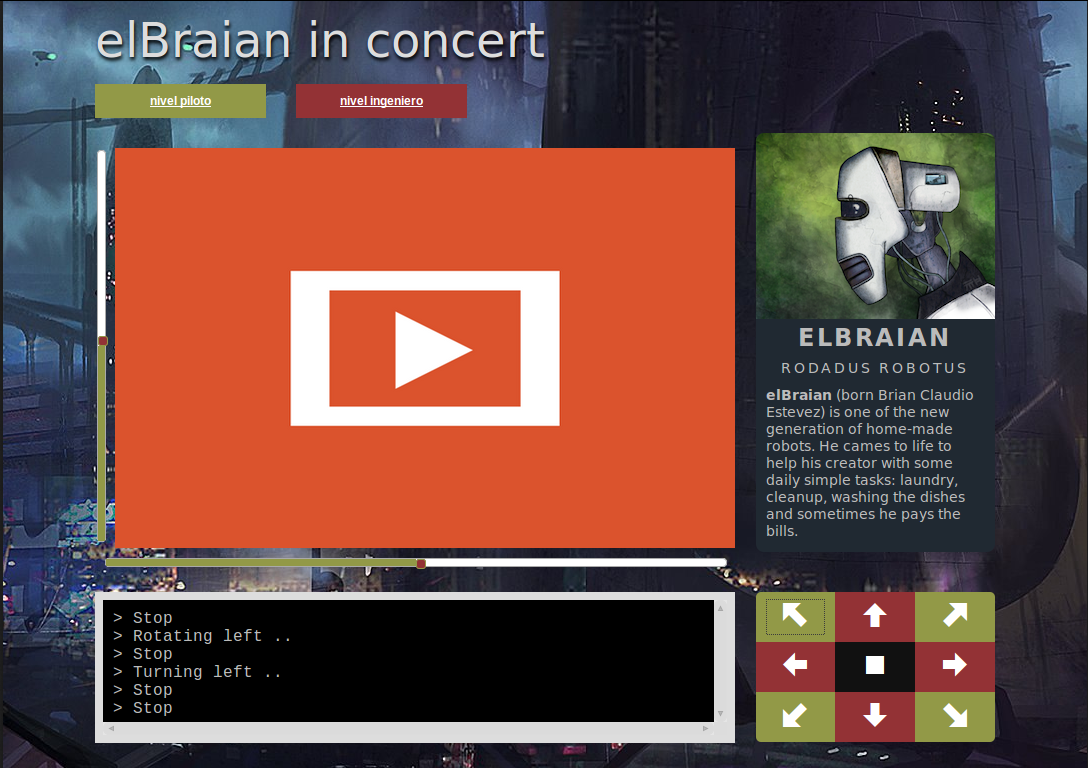
\includegraphics[width=0.5\textwidth]{figures/elbrian-1}
    \caption{Pantalla principal de elBrian (en el recuadro rojo normalmente
        se muestra la cámara de el robot)}
    \label{fig:elbrian}
\end{figure}

Las tecnologías utilizadas en la interfaz web de ``elBrian'' coinciden en gran
parte con las utilizadas en el desarrollo de XRemoteBot, pero el objetivo del
servidor de ``elBrian'' es controlar un único robot en un ambiente local.
Además este servidor
se instala en el robot utilizado,  cuestión que sería imposible en los
robots basados en
microcontroladores AVR y PIC (``Basic Stamp 2`` de Parallax)
a los que XRemoteBot se encuentra dirigido.

%FIXME: fijate de poner aunque sea notas al pie con las referencias de los paquetes o protocolos que nmbras... el que no sabe.. se muere...

El servidor web de ``elBrian'' está implementado usando el framework
Tornado\footnote{\url{http://www.tornadoweb.org/}},
WebSockets\footnote{\url{http://www.websocket.org/}},
mjpg-streamer\footnote{\url{https://github.com/jacksonliam/mjpg-streamer}},
opencv\footnote{\url{http://opencv.org/}}
y JSON\footnote{\url{http://json.org/}}.
El mismo está diseñado para ejecutarse
en el robot ya que el mismo está basado en una placa RaspberryPi, la cuál
cuenta con un procesador ARM perfectamente capaz de ejecutar un sistema
operativo completo como GNU/Linux y de soportar el intérprete oficial de Python.

Mientras que este servidor coincide en gran medida en la elección de lenguaje
y bibliotecas utilizadas, su implementación es específica para el robot ``elBrian''
y no puede ser portada a robots con menores capacidades de procesamiento
sin una reescritura significativa. Además el protocolo utilizado no contempla
el acceso a valores de sensores siendo los únicos mensajes que permite enviar
al robot los comandos de movimientos.

Referencias del proyecto:
\begin{itemize}
    \item Página del proyecto: \url{http://www.educabot.org/}
    \item Código fuente de ``elBrian'': \url{https://github.com/educabot/elBraian}
\end{itemize}

\section{Gobot con cppp-io}

Gobot\footnote{\url{http://gobot.io}}
es una biblioteca que permite controlar robots programando en el lenguaje
Go\footnote{\url{https://golang.org/}}. Esta biblioteca soporta el
protocolo Firmata
para controlar robots
conectados directamente a través de una interfaz serial, como es el caso
de los robots Multiplo N6, y soporta la API
cppp-io\footnote{\url{https://github.com/hybridgroup/cppp-io/}}
que define una API JSON
que permite el acceso a la información y control de robots a través de la Web.

Gobot además tiene compatibilidad con distintos sensores y robots, además de
ser compatible con
placas utilizadas normalmente en la construcción de robots como Arduino,
Raspberry Pi, Intel Edison y Beaglebone Black%
\footnote{\url{http://gobot.io/\#platforms}}.

Este proyecto es interesante como base para desarrollar algún proyecto
similar a XRemoteBot en Go, pero requiere además la reimplementación
del módulo de Python DuinoBot que controla, a través de una versión
modificada del protocolo Firmata, a los robots Multiplo N6. Por otro
lado, los robots Scribbler tampoco aparecen en la lista de robots soportados.

Referencias del proyecto:
\begin{itemize}
    \item Página del proyecto: \url{http://gobot.io}.
    \item Protocolo de su API Web: \url{https://github.com/hybridgroup/cppp-io/}.
\end{itemize}


\section{Cylon.js}

Cylon.js es un proyecto hermano de Gobot y soporta la misma variedad
de dispositivos y también provee una API cppp-io, con la diferencia
de que la biblioteca provista está escrita en Javascript para NodeJS.

Una característica interesante de Cylon.js es que soporta distintos
protocolos para su API remota como ser HTTP, socket.io y la capacidad
de agregar nuevos protocolos con
plugins

\begin{lstlisting}[caption={Cylon.js controlando 2 robots ``sphero'' usando HTTP},
label={lst:cylonjs_ejemplo}]
"use strict";

var Cylon = require("cylon");

// ensure you install the API plugin first:
// $ npm install cylon-api-http
Cylon.api({
  host: "0.0.0.0",
  port: "8080"
});

var bots = {
  "Thelma": "/dev/rfcomm0",
  "Louise": "/dev/rfcomm1"
};

Object.keys(bots).forEach(function(name) {
  var port = bots[name];

  Cylon.robot({
    name: name,

    connections: {
      sphero: { adaptor: "sphero", port: port }
    },

    devices: {
      sphero: { driver: "sphero" }
    },

    work: function(my) {
      every((1).seconds(), function() {
        console.log(my.name);
        my.sphero.setRandomColor();
        my.sphero.roll(60, Math.floor(Math.random() * 360));
      });
    }
  });
});

Cylon.start();
\end{lstlisting}

En el código~\ref{lst:cylonjs_ejemplo} se puede ver un ejemplo de
Cylon.js del lado del servidor exponiendo dos robots de tipo
\textit{sphero} a través de la API HTTP,
una vez ejecutado este código en el servidor, a través de la API se
les podrá enviar un mensaje a los robots
robots que hará que cambien
de color
y se desplacen
rodando\footnote{Los robots sphero son pequeñas esferas \url{http://www.gosphero.com/}.}.

Si bien en la documentación del proyecto se detalla como habilitar
un sistema de login para acceder a la API de forma remota, el mismo
no parece estar diseñado para el acceso concurrente de distintos usuarios
ya que de la documentación no surge que Cylon.js soporte un sistema
de reserva de robots o de exclusión mutua en el acceso a los mismos.

Referencias del proyecto:
\begin{itemize}
    \item Página del proyecto: \url{http://cylonjs.com/}.
\end{itemize}


\section{VCar}

\begin{figure}
    \centering
    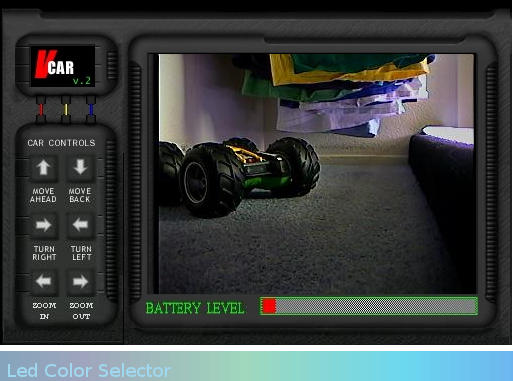
\includegraphics[width=0.5\linewidth]{figures/vcar}
    \caption{Interfaz de VCar}
    \label{fig:vcar}
\end{figure}

VCar es un auto a control remoto, cuyo control fue modificado para
se manipulado por software desde  una computadora con GNU/Linux la
cuál permite controlar el robot de forma remota y verlo
a través de una cámara de
video\footnote{\url{http://www.hellspark.com/new/css/vcar/vcar.html}}
(figura~\ref{fig:vcar}).
El acceso al robot es público
aparentemente sin ningún tipo de restricción y la página
si bien no tiene detalles de todo el hardware y el software utilizados
provee algunas fotos de la construcción del
sistema\footnote{\url{http://www.hellspark.com/dm/gallery2/v/projects/robotics/vcar/}}

Referencias del proyecto:
\begin{itemize}
    \item Página del proyecto: \url{http://www.hellspark.com/new/css/vcar/vcar.html}.
    \item Galería de fotos: \url{http://www.hellspark.com/dm/gallery2/v/projects/robotics/vcar/}}
\end{itemize}


\section{Tele Toyland}

Tele Toyland\footnote{\url{http://www.teletoyland.com}} es un sitio que provee acceso a varios dispositivos a través de una interfaz
web. Por ejemplo, es posible controlar un cabezal con una punta que dibuja sobre
una caja de arena. Basta con hacer clic sobre las posiciones sobre las cuales
se quiere que pase la punta y presionar el botón ``go'' para que el cabezal
empiece a moverse dibujando lo pedido. En éste y el resto de los experimentos
disponibles en el sitio, los resultados se pueden ver a través de un streaming
de video.

Entre los proyectos con los que permite interactuar Tele Toyland
se encuentran  2 areneros como el descripto
anteriormente, una torre de leds, una marioneta y laberintos.

El sitio no provee detalles del software, ni el protocolo utilizado. Desde
lo funcional
provee una especie de control remoto para los distintos dispositivos a los
que permite
manipular, en donde se puede, incluso, configurar una serie de instrucciones a ejecutar
en secuencia. Sin embargo no provee una biblioteca que permita controlar
los dispositivos desde un lenguaje de programación.

Referencias del proyecto:
\begin{itemize}
    \item Página del proyecto: \url{http://www.teletoyland.com}.
\end{itemize}
% FIXME
%\section{}
%http://www3.uji.es/~pnebot/Files/Articuls/RemoteProgramming.pdf
%Otro
%http://telerobot.mech.uwa.edu.au/Telerobot/instructions.html
\section{Otros proyectos}
% www.linuxuser.co.uk/tutorials/control-your-raspberry-pi-robot-from-a-web-connected-device



%FIX ME ESTO QUEDA MUY DESCOLGADO..... yo pondŕia algo como 
%Bajo la consigna DIY, o ``do it yourself'' y acá poner un par de ref!!!, existen diversas.....y seguir...., 

Existieron otros sistemas similares en el pasado, pero actualmente se
encuentran fuera de línea por problemas técnicos o bien porque el
experimento terminó como por ejemplo
``TU Freiberg Robotics''\footnote{\url{www.informatik.tu-freiberg.de/\~frobots/}}
que permitía controlar robots en una mini cancha de fútbol,
``WebTruck''\footnote{\url{http://www.webtruck.org/cinteraction_html}} que
permitía controlar distintos vehículos.

También existen otros proyectos que requieren instalar software extra
como ``The UWA Telerobot'' que requiere instalar software propietario
y crear una cuenta para ser utilizado, este proyecto permite controlar
un brazo robótico en un taller.

Finalmente en la consigna de ``do it yourself'' existen diversas guías para
programar servidores que permitan controlar robots o microcontroladores
en general, se puede encontrar un caso muy bien explicado en el sitio
de Adafruit~\url{https://learn.adafruit.com/wifi-controlled-mobile-robot/building-the-web-interface},
este es un buen ejercicio de programación, sobre todo para aprender a
programar servidores que provean una API web y clientes que la consuman. Sin
embargo estas guías son introductorias y el objetivo es crear un servidor
muy simple, similar a lo que fue el servidor RemoteBot, pensados para ser
usados en un ambiente local ya que no proveen autenticación en general.

\section{Conclusiones del capítulo}

Si bien existen proyectos parecidos que brindan al público la posibilidad
de controlar un robot de manera remota, ninguno de estos es una solución
completa al problema de enseñar a programar usando
robots de forma remota y permitiendo a distintos usuarios reservar
temporalmente distintos
robots de forma que no haya conflicto en la interacción entre los usuarios.

%\chapter{Arquitecturas}\label{cha:arquitectura}
\chapter{Myro y Duinobot: Las bases de la propuesta}\label{cha:arquitectura}

%FIX ME: yo pondría como titulo: Myro y DuinoBot: LAS BASES DE LA PROPUESTAS

%El capítulo 2 describe la arquitectura de DuinoBot, Myro, Remotebot y
%XRemoteBot detallando las mejoras provistas por XRemoteBot.

% FIXME: QUIZAS ESTE CAPITULO PODRÍA IR ANTES DEL ANTERIOR... YA QUE SEGURAMENTE VAS A NOMBRAR Y DESCRIBIR VARIAS COSAS QUE LUEGO NOMBRAS ALLÁ... FIJATE

Tanto Remotebot como XRemoteBot tienen arquitecturas complejas que
dependen de otras librerías y de software instalado en los robots.
El objetivo de este capítulo es describir la interacción entre los
distintos dispositivos y aplicaciones utilizadas, demarcando el límite
entre el desarrollo realizado para esta tesina, XRemoteBot, con el software ya
existente con el que interactúa.

\section{Myro}\label{sec:myro}

Como se mencionó al comienzo de este informe,
Myro\footnote{\url{http://myro.roboteducation.org/}}
es la biblioteca utilizada para controlar a los robots
``Scribbler''\footnote{\url{http://wiki.roboteducation.org/Myro_Hardware}}
desde un script Python. Esta biblioteca fue desarrollada por
Institute for Personal Robots in Education (IPRE) y
y utilizado en el proyecto Robot en la enseñanza de ciencias
de la computación\footnote{\url{http://www.roboteducation.org}}
en distintos niveles
educativos\footnote{\url{http://www.roboteducation.org/schools.html}}.
Si bien el proyecto original fue desarrollado por Microsoft Research,
el software generado es software libre y portable tanto en sistemas Windows
como GNU/Linux.


Myro puede interactuar con los robots de dos
formas diferentes: a través de un cable serial (RS323) o bien usando bluetooth
con RFCOMM. El funcionamiento de Myro requiere que el robot tenga
cargado un firmware determinado que espera las instrucciones desde el puerto
serial con el que cuenta el robot y una placa llamada FLUKE-6 que se conecta
al puerto serial del robot y cuenta con un adaptador bluetooth que permite
enviarle comandos de forma inalámbrica a través de este protocolo.

\begin{figure}
    \centering
    \includegraphics[width=.7\textwidth]{figures/diagrama_myro}
    \caption{Diagrama de bloques de Myro}
    \label{fig:diagrama_myro}
\end{figure}

La figura~\ref{fig:diagrama_myro} muestra la interacción entre los componentes
más importantes de software y hardware desde el script del usuario hasta el
robot.

Cabe destacar que el código de Myro funciona con Python 2.7 pero no con
Python 3, posiblemente esto se relacione con la desición del \ipre{}
de desarrollar una nueva biblioteca para controlar a los robots que funcione
en distintos lenguajes de
programación\footnote{\url{http://calicoproject.org/}}. De todas formas se
decidió seguir con Myro por la experiencia del autor de esta tesina
con esta librería.

% FIXME Maybe más adelante
Lamentablemente el servidor SVN oficial donde se publicaban las
actualizaciones de Myro a la fecha de escribir este documento
no se encuentra en funcionamiento, por lo que debí recurrir a una
copia de este repositorio en
GitHub\footnote{\url{https://github.com/yingted/Myro}} de la cuál
cree un fork y la reorganicé de forma tal que fuera posible instalar
esta librería desde un entorno Python con un solo comando y hice
una pequeña corrección para que el uso de la biblioteca IDLE sea
opcional ya esa biblioteca sirve para crear interfaces gráficas
y eso no es necesario para este proyecto.

Esta librería (técnicamente un paquete Python) consta de múltiples
módulos y requiere de otros para contar con funcionalidades opcionales
como el soporte de Joysticks, una interfaz gráfica para mostrar
los valores de los sensores en un diálogo y soporte para manipulación
de imágenes para poder sacar fotos con el robot y manipularlas. Sin
embargo para el alcance de este trabajo con el acceso a las funcionalidades
básicas del robot como moverlo y acceder a sus sensores es suficiente.


\section{DuinoBot}\label{sec:duinobot}

La biblioteca de Python
DuinoBot\footnote{\url{https://github.com/Robots-Linti/duinobot}}
desarrollada en conjunto entre un grupo
de becarios del laboratorio LINTI de esta Facultad y la empresa RobotGroup
cuenta con un modo de operación similar al de Myro, conectándose con
los robots a través de un dongle XBee (que utiliza el protocolo ZigBee)
conectado a través de un puerto USB con el dispositivo controlante.
Para que esta biblioteca pueda controlar a los robots estos últimos
deberán tener instalado también un firmware especial: en este caso,
es un una versión modificada de un firmware que implementa el protocolo
Firmata de uso amplio para controlar dispositivos Arduino a través de una
interfaz serial que habitualmente es el puerto USB, pero en este caso
la interfaz serial está conectada a un dongle XBee en el robot, la interacción
entre las distintas capas de software y hardware se ilustra en la
figura~\ref{fig:funcionamiento_duinobot_diagrama}.

\begin{figure}
    \centering
    \begin{subfigure}[b]{0.7\textwidth}
        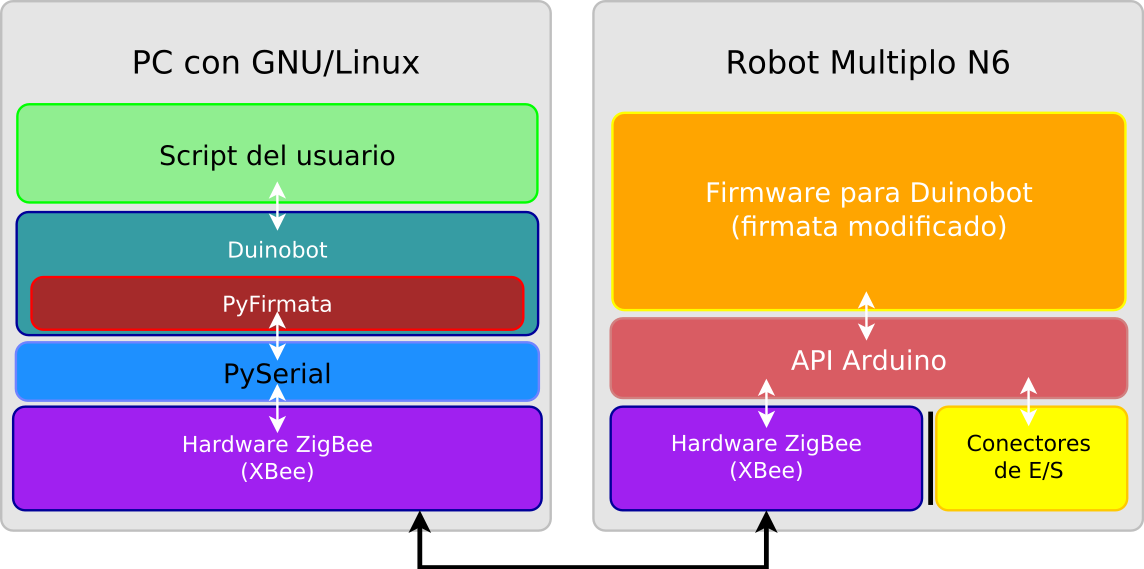
\includegraphics[width=.95\textwidth]{figures/diagrama_duinobot}
        \subcaption{Diagrama de bloques de DuinoBot}
        \label{fig:funcionamiento_duinobot_diagrama}
    \end{subfigure}
    \begin{subfigure}[b]{0.29\textwidth}
        \includegraphics[width=\textwidth]{figures/arquitectura_actual}
        \subcaption{Esquema de conexión típico}
        \label{fig:funcionamiento_duinobot_conexion}
    \end{subfigure}
    \caption{Funcionamiento de DuinoBot}
    \label{fig:funcionamiento_duinobot}
\end{figure}

La modalidad de uso esperada con DuinoBot consiste en que cada usuario
debe contar con una computadora, conectada por USB a un dongle XBee,
y desde esa computadora puede controlar uno o más robots. Con esa modalidad
fueron utilizados los robots en los cursos del proyecto
``Programando con robots y software libre'' y en actividades similares
planteadas posteriormente, generalmente además cada alumno controla
un único robot, el esquema de conexión típico en estos cursos se encuentra
ilustrado en la figura~\ref{fig:funcionamiento_duinobot_conexion}.


% El capítulo 4 describe la implementación de los clientes y el modo de uso
% de cada uno destacando algunas diferencias y decisiones de diseño en la
% implementación en Javascript.

\chapter{Implementación de los clientes}\label{ch4}
Los clientes hosted no tienen video % FIXME
Cuestiones de estilo casing copiando duinobot

Se implementaron 3 clientes para permitir el uso de XRemoteBot desde 3
lenguajes de programación distintos: Python, Ruby y Javascript. Este último
en el navegador.

\section{Cliente Python}\label{ch4:python}
El uso del cliente Python es muy similar al uso directo de los robots con la
biblioteca DuinoBot aunque la implementación es bastante diferente por el protocolo
subyacente.

El cliente Python utiliza un solo módulo que no pertenece a la biblioteca estándar
de Python, el módulo para acceso a WebSockets
\textit{websocket-client}~\footnote{\url{https://pypi.python.org/pypi/websocket-client}}
que cuenta, además de con una interfaz asincrónica, con una interfaz de ``bajo nivel''
sincrónica similar a la interfaz tradicional de Sockets.

\begin{lstlisting}[language=Python,
caption={Ejemplo con XRemoteBot para Python},label=lst:ejemplo_xremotebot_python]
from xremotebot import *
server = Server('ws://xremotebot.example:8000/api', 'api_key')
robot = server.fetch_robot()
robot.forward(100, 1)
robot.backward(50, 2)
print(robot.getObstacle())
\end{lstlisting}


Las operaciones con demoras, como los movimientos se implementan localmente
utilizando 2 mensajes y la función \texttt{time.wait()} de Python. De esta
forma
invocar al método \texttt{robot.forward(100, 1)} se traduce en los mensajes
de
la figura~\ref{fig:mensajes_xremotebot_python_json}. Como todos los métodos
de movimiento
proveen esta funcionalidad de demora, la misma implementada en el
\textit{decorator}~\footnote{Esto es un decorator de Python, no confundir
con el patrón de diseño. \url{https://www.python.org/dev/peps/pep-0318/}}
\texttt{xremotebot.timed} a fin de evitar repetición de código.

\begin{lstlisting}[language=Python,
caption={Mensajes generados al invocar \texttt{robot.forward(100, 1)} en
XRemoteBot para Python}, label=lst:ejemplo_xremotebot_python_json]
{
    "entity": "robot",
    "method": "forward",
    "args": [100]
}
# Después de 1 segundo...
{
    "entity": "robot",
    "method": "stop",
    "args": []
}
\end{lstlisting}


\section{Cliente Ruby}\label{ch4:ruby}

Las gemas que proveen soporte para WebSockets en Ruby proveen una API
asincrónica que no es deseable para este proyecto por lo que me incliné
por incorporar el código del
proyecto~\footnote{\url{https://github.com/gimite/web-socket-ruby}}
al cliente Ruby de XRemoteBot, este proyecto no se encuentra empaquetado
en forma de gema pero provee una API sincrónica que permite implementar
el cliente Ruby de XRemoteBot para que se comporte de una forma muy similar
a la biblioteca DuinoBot original.

\begin{lstlisting}[language=Ruby,
caption={Ejemplo usando XRemoteBot para Ruby},
label=lst:ejemplo_xremotebot_ruby]
require 'xremotebot'
server = XRemoteBot::Server.new('ws://xremotebot.example:8000/api',
                                'api_key')
robot = server.fetch_robot
robot.forward 100, 1
robot.backward 50, 2
print robot.getObstacle
\end{lstlisting}



\section{Cliente Javascript}\label{ch4:javascript}

\subsection{API Javascript y asincronismo}
Como se mencionó con anterioridad, gran parte de las decisiones de diseño de XRemoteBot
se hicieron para permitir la implementación de un cliente Javascript, pero dado el hecho
de que Javascript dentro del entorno de un navegador Web se comporta de forma asincrónica
no fue posible implementar un cliente Javascript cuyo uso se asemeje al de la biblioteca
de Python DuinoBot.

Para ilustrar esta problemática se puede tomar en consideración el 
código~\ref{lst:ejemplo_duinobot}
típico hecho usando DuinoBot en Python y analizar los inconvenientes para replicar
algo similar en Javascript.

\begin{lstlisting}[language=Python,
caption={Ejemplo típico usando DuinoBot},label=lst:ejemplo_duinobot]
from duinobot import *
board = Board()
robot = Robot(board, 10)
robot.forward(100, 1)
robot.backward(50, 2)
print(robot.getObstacle())
\end{lstlisting}


Las líneas 2 y 3 del ejemplo de la código~\ref{lst:ejemplo_duinobot} son
operaciones que retornan objetos, en XRemoteBot la línea 2 no tiene sentido
ya que la placa a la que está conectado el robot está predefinida en el
servidor, pero la línea 3 sí es necesaria para obtener una instancia de un
robot no reservado, estas operaciones que retornan un valor el XRemoteBot
se dividen en un mensaje de petición y uno de respuesta, el problema
es que por el asincronismo de Javascript y de la API de WebSockets no
es posible determinar en que momento llegará la respuesta con el valor
retornado y la única forma de bloquear la ejecución del script hasta que
llegue la respuesta sería hacer ``busy waiting'', lo cuál puede llegar a
bloquear la pestaña del navegador ya que los navegadores típicamente usan
un solo thread compartido entre el renderizado de la página, manejo de
eventos y ejecución del código Javascript asociado a la página.

En tanto las líneas 4 y 5 si bien no retornan un valor deben ejecutarse
en orden, y la línea 5 en este caso debe ejecutarse precisamente 1 segundo
después de la ejecución de la línea 4, también la línea 6 deberá ejecutarse
2 segundos después de la línea 5 ya que no es lo mismo preguntar si hay
un obstáculo cuando el robot aún no retrocedió, esto que parece muy obvio
y natural en la mayoría de los lenguajes de programación no es posible
en Javascript (dentro del navegador, con intérpretes como NodeJS sí es
posible) y el orden de ejecución y demora no se puede lograr simplemente
poniendo una instrucción debajo de otra.\footnote{FIXME}


La solución encontrada a este problema fue el uso de
\textit{Promises}~\citep{ECMA-262},
las \textit{Promises} proveen un mecanismo para ejecutar instrucciones,
que dependen de los resultados o de la terminación de eventos asincrónicos,
las \textit{Promises} permiten tener secuencia e interdependencia entre los
mensajes enviados a los
robots.
Si bien el objeto \textit{Promise} está en proceso de estandarización,
los navegadores Google Chrome, Firefox, Internet Explorer, Opera y Safari las
soportan~\footnote{\url{https://developer.mozilla.org/en-US/docs/Web/JavaScript/Reference/Global_Objects/Promise}}.
El problema de esta solución es que la sintaxis de un script XRemoteBot en
Javascript usando \textit{Promises}
resulta bastante distinta de la sintaxis de un script DuinoBot como resulta
evidente
en el código~\ref{lst:ejemplo_xremotebot_javascript} donde se muestra un
script equivalente
al del código~\ref{lst:ejemplo_duinobot} escrito en Javascript.

\begin{lstlisting}[language=C,
caption={Ejemplo de XRemoteBot en Javascript},
label=lst:ejemplo_xremotebot_javascript]
var server = new Server('xremotebot.example:8000', 'api-key');
server.onConnect(function(){
    server.fetch_robot().then(function(robot){
        robot.forward(100, 1).then(function(){
            robot.backward(50, 2).then(function(){
                robot.getObstacle().then(function(obstacle){
                    println(obstacle);
                })
            })
        })
    });
});
\end{lstlisting}

Como se puede ver después de cada acción bloqueante, es decir cada método que
provoque una demora, y de cada método que retorne un valor útil, como
\texttt{Robot\#getObstacle()}, se invoca el método \texttt{Promise\#then()} con
una función anónima como argumento. Esta función que se pasa por argumento al
then se ejecutará si la \textit{Promise} se ``resuelve'', en el caso de
XRemoteBot la \textit{Promise} se ``resuelve'' cuando el servidor
responde al mensaje que generó la \textit{Promise}.
Este mecanismo se logró identificando cada mensaje con un \texttt{msg\_id},
manteniendo un objeto Javascript (usado como si fuera un \texttt{dict}
o \texttt{HashMap}) con el identificador como clave y la promesa
correspondiente a cada uno los mensajes cuyas respuestas están pendientes
como valor. Dentro del callback \texttt{onmessage} del WebSocket utilizado
al recibir una respuesta se busca el \texttt{msg\_id} en el objeto de
mensajes con respuesta pendiente y se ``resuelve'' la promesa correspondiente
a este mensaje. De esta manera se ejecuta la siguiente función (pasada como
argumento a \texttt{Promise\#then}) siguiendo con el flujo del programa
en orden y con la demora necesaria. En el
código~\ref{lst:ejemplo_xremotebot_javascript_promises} se muestra esta primer
implementación.


\begin{lstlisting}[language=C,
caption={Ejemplo simplificado de la implementación de XRemoteBot con
Promises dentro del constructor Server en remotebot.js},
label=lst:ejemplo_xremotebot_javascript_promises]
this.send_ws_msg = function(msg){
    var promise;
    promise = new Promise(function(resolve, reject){
        that.pending_msgs[msg_id] = {resolve: resolve, reject: reject};
    });
    msg['msg_id'] = msg_id;
    that.ws.send(JSON.stringify(msg));
    return promise;
}
// ...
this.ws.onmessage = function(msg){
    msg = JSON.parse(msg.data);
    if (msg['msg_id'] !== undefined){
        var executor = that.pending_msgs[msg['msg_id']];
        delete that.pending_msgs[msg['msg_id']];
        executor.resolve(msg);
    }
};
\end{lstlisting}


Evidentemente esta forma de programar resulta engorrosa y poco práctica,
por lo que se añadieron
lógica y estructuras de datos extra que serializan en envío de mensajes al
servidor, enviando de a un mensaje por vez (el objeto Javascript con
mensajes con respuesta pendiente tendrá a lo sumo una entrada)
y encolando los mensajes sobrantes
en una cola de mensajes demorados (\texttt{Server\#delayed}), cuando
el servidor contesta el mensaje enviado anteriormente se toma un mensaje
de la cola si lo hubiere y se lo envía al servidor. De esta manera
se garantiza la demora necesaria entre la ejecución de cada método
del robot, sin embargo para obtener los valores de retorno de los métodos,
como en el caso de los métodos de acceso a los sensores, sigue siendo
necesario el uso del método \texttt{Promise\#then}. A pesar de esto último
como se puede ver en el código~\ref{lst:ejemplo_xremotebot_javascript_cola}
con estas modificaciones es posible hacer que el cliente Javascript
tenga una API más limpia y usable, esta última versión es la definitiva
para este trabajo.

\begin{lstlisting}[language=C,
caption={Ejemplo de XRemoteBot en Javascript con empleo de una cola para
serializar mensajes},
label=lst:ejemplo_xremotebot_javascript_cola]
var server = new Server('xremotebot.example:8000', 'api-key');
server.fetch_robot().then(function(robot){
    robot.forward(100, 1);
    robot.backward(50, 2);
    robot.getObstacle().then(function(obstacle){
        println(obstacle);
    });
});
\end{lstlisting}


Una solución alternativa para lograr imitar tanto como sea posible la
API de DuinoBot puede ser utilizar un intérprete Javascript implementado en
Javascript como
JS-Interpreter~\footnote{\url{https://github.com/NeilFraser/JS-Interpreter}},
pero requeriría modificar el intérprete para lograr una ejecución paso a paso
controlada por el flujo de mensajes a través de la conexión con WebSockets,
además de agregar complejidad, este tipo de intérpretes no accede a un entorno
compreto como lo hace el intérprete incorporado en los navegadores y puede
tener incompatibilidades o funcionalidades no implementadas, en este caso
por ejemplo JS-Interpreter no soporta interrupciones y no puede interactuar
directamente con DOM, otra opción es
Hypnotic~\footnote{\url{http://coolwanglu.github.io/hypnotic/web/demo.html}}
que utiliza el intérprete Narcissus y provee una función \tt{sleep()} que
demora la ejecución del código como se desea para este proyecto, pero el
invoveniente de Hypnotic es que por el momento solamente funciona en el
navegador
Firefox~\footnote{\url{https://github.com/coolwanglu/hypnotic/wiki\#limitations}}.


\subsection{Interacción con DOM y JQuery}

\subsection{Interfaz Web y streaming de video}

La interfaz Web de XRemoteBot, que está pensada principalmente para los casos
de uso donde los clientes están en una ubicación geografica distinta a la de
los robots provee login, acceso a la visualización y renovación de una
clave alfanumérica única por cada usuario denominada \textit{API key} que
permite reservar y controlar los robots sin la necesidad de exponer el nombre
de usuario y contraseña, y una página que permite ver los robots en vivo por
video opcionalmente controlandolos con un script Javascript.

Login y renovación de API, doc

La interfaz web pensada para ser utilizada en conjunto con el cliente
Javascript (aunque puede ser accedida sin problemas aún si se usa
otro de los clientes) provee un area de texto para escribir el script
a ejecutar % FIXME
para la misma se utilizó CodeMirror ...

Un area de texto que simula la salida de una terminal, en la misma
se pueden ver mensajes de log generados con la función
\texttt{rblog} que pueden ser habilitados o deshabilitados desde un
checkbox y mensajes impresos con la función \texttt{rbprintln}.

Un area de video destinada a emisiones en vivo que muestren la posición
del robot, el mismo no requiere ningún plugin ya que se utilizó
\texttt{jsmpeg}~\footnote{\url{https://github.com/phoboslab/jsmpeg}}
que permite emitir video en vivo usando WebSockets y renderizarlo
en el navegador en un elemento Canvas, de esta manera se logró tener
video en vivo utilizando características estándar de HTML5.

\appendix
% Apéndice A Serialización

\chapter{Serialización}
\label{ch:serializacion}

Siendo una aplicación cliente-servidor remotebot requiere algún método de
serialización para intercambiar datos entre los clientes y el servidor,
considerando que el servidor no es más que un servidor web que usa websockets
como protocolo, el método de serialización más adecuado parece ser JSON
(Javascript Serialization Object Notation).

JSON cuenta con las siguientes características:

\begin{enumerate}
    \item Es un formato estandarizado por ECMA~\citep{ecma-404}
        y está especificado por la rfc-7159~\citep{rfc-7159}.
    \item Soporta los tipos de datos necesarios para intercambiar mensajes con
        los datos necesarios para controlar los robots usando un nivel de
        abstracción adecuado.
    \item Al ser un formato de texto es simple analizar el tráfico entre los
        clientes y el servidor para detectar posibles errores.
    \item Está soportado de forma nativa por los navegadores más
        utilizados%~\footnote{\url{http://caniuse.com/#search=json}}.
\end{enumerate}

Pero también existen otras alternativas cuyos objetivos son serialización
y de-serialización rápida, y datos serializados más compactos
como BSON (Binary JSON) y (CBOR Concise Binary Object Representation).

Algunas características de BSON y CBOR son:

\begin{enumerate}
    \item Codifican la información en formato binario.
    \item Son tan fáciles de usar como JSON.
    \item Ambos formatos proveen un superset de los tipos de datos provistos
        por JSON.
    \item CBOR está especificado por la rfc-7049~\citep{rfc-7049}.
    \item BSON tiene una especificación informal pero cuenta una
        implementación bien conocida siendo la representación de datos primaria en
        MongoDB~\footnote{\url{http://bsonspec.org/}}.
    \item Por estar en formato binario decodificar una captura de tráfico
        para depurar un programa es más laborioso.
    \item En algunos casos estos formatos binarios generarán mensajes más
        chicos que JSON, pero no siempre.
    \item Requieren usar librerías Javascript en los clientes web ya que los
        navegadores no lo implementan de forma nativa.
\end{enumerate}

Para tomar un decisión respecto al formato a utilizar se decidió generar
16 archivos \texttt{JSON} con datos aleatorios, estos archivos se cargaron
con una cantidad de entradas múltiplo de 1024 desde 1024 hasta 16384, donde
cada una de estas entradas es un objeto \texttt{JSON} con 5 entradas de tipo
numérico, 5 strings, 5 objetos (cada uno con una entrada numérica) y 5
arrays (cada uno con 2 entradas de tipo string).

Estos archivos se cargaron desde scripts similares en Python y Javascript que
de-serializaron y serializaron estos datos repetidas veces calculando el tiempo
promedio que llevó hacer cada una de estas acciones para cada formato.

Se eligió hacer las pruebas con Python y Javascript porque el primero es el
lenguaje de implementación del servidor y del cliente que probablemente tenga
más uso en un futuro, mientras que Javascript es el lenguaje de implementación
del cliente que se ejecutará en los navegadores web y que puede servir como
base para implementaciones con Brython, Skulp, Opal, etc...

Para hacer el experimento repetible la implementación en
Javascript se ejecutó con el intérprete \textbf{nodejs} basado en
el motor \textbf{v8} usado por \textbf{Chrome} y además se crearon
scripts de apoyo para generar los datos de prueba, ejecutar los scripts
con los distintos formatos de forma automatizada y formatear los datos
resultantes en archivos csv.

Todas las pruebas se realizaron sobre Lihuen 6 beta (basado en Debian Jessie)
en una notebook con procesador ``Intel(R) Core(TM) i3 CPU M 370 @ 2.40GHz''
y 4GB de RAM % NOTA: son 4GB no 4GiB
usando Python 3.4.2 y NodeJS 0.10.35~\footnote{Se usó NodeJS 0.10.35 ya que
la versión 0.10.29 distribuida al momento con Debian Jessie tenía un bug que
generaba un error de memoria al
deserializar strings largos con \texttt{JSON.load} (CVE-2014-5256)}

De estas pruebas se desprenden las mediciones de las
figuras~\ref{fig:ser-time-py}, \ref{fig:ser-time-js} y \ref{fig:ser-size}.

\begin{figure}
    \centering
    \begin{framed}
        \begin{tikzpicture}[trim axis left, trim axis right]
            \begin{axis}[
                    height=10cm,
                    width=10cm,
                    scaled x ticks = false, % No usar notación exponencial
                    xlabel=Cantidad de entradas,
                    ylabel=Segundos,
                    x tick label style={/pgf/number format/fixed, rotate=45, anchor=north east}, % Las etiquetas son números y rotar 45°
                    xtick=data, % Generar una etiqueta por punto en los datos
                    ylabel near ticks, % Poner las etiquetas más o menos cerca de algunos datos
                    ymin=0, % No hay tiempos negativos
                    xmin=1024, % La escala empieza en 1024
                    legend style={legend pos=north west}, % Cuadro de leyendas a la derecha arriba
                    every axis x label/.style={
                        at={(axis description cs:0.5,-0.15)}, % Desplazar la descripción del eje x
                        anchor=north, % El desplazamiento relativo a la parte superior del texto
                    },
                    legend cell align=left, % Alineación del texto en la caja de leyendas
                ]
                \foreach \s in {json, bson, cbor} {
                    \addlegendentryexpanded{\s\ dump}
                    \addplot table [x=entries, y=dump_time, col sep=comma] {data/py-\s.csv};

                    \addlegendentryexpanded{\s\ load}
                    \addplot table [x=entries, y=load_time, col sep=comma] {data/py-\s.csv};
                }
            \end{axis}
        \end{tikzpicture}
    \end{framed}

    \caption{Cantidad de entradas versus tiempo de serialización y deserialización en Python}
    \label{fig:ser-time-py}
\end{figure}

\begin{figure}
    \centering
    \begin{framed}
        \begin{tikzpicture}[trim axis left, trim axis right]
            \begin{axis}[
                    height=10cm,
                    width=10cm,
                    scaled x ticks = false, % No usar notación exponencial
                    xlabel=Cantidad de entradas,
                    ylabel=Segundos,
                    x tick label style={/pgf/number format/fixed, rotate=45, anchor=north east}, % Las etiquetas son números y rotar 45°
                    xtick=data, % Generar una etiqueta por punto en los datos
                    ylabel near ticks, % Poner las etiquetas más o menos cerca de algunos datos
                    ymin=0, % No hay tiempos negativos
                    xmin=1024, % La escala empieza en 1024
                    legend style={legend pos=north west}, % Cuadro de leyendas a la derecha arriba
                    every axis x label/.style={
                        at={(axis description cs:0.5,-0.15)}, % Desplazar la descripción del eje x
                        anchor=north, % El desplazamiento relativo a la parte superior del texto
                    },
                    legend cell align=left, % Alineación del texto en la caja de leyendas
                ]
                \foreach \s in {json, bson, cbor} {
                    \addlegendentryexpanded{\s\ dump}
                    \addplot table [x=entries, y=dump_time, col sep=comma] {data/js-\s.csv};

                    \addlegendentryexpanded{\s\ load}
                    \addplot table [x=entries, y=load_time, col sep=comma] {data/js-\s.csv};
                }
            \end{axis}
        \end{tikzpicture}
    \end{framed}
    \caption{Cantidad de entradas versus tiempo de serialización y deserialización en Javascript (nodejs)}
    \label{fig:ser-time-js}
\end{figure}


\begin{figure}
    \centering
    \begin{framed}
        \begin{tikzpicture}[trim axis left, trim axis right]
            \begin{axis}[
                    height=10cm,
                    width=10cm,
                    scaled x ticks = false,
                    xlabel=Cantidad de entradas,
                    ylabel=Tamaño en MiB,
                    x tick label style={/pgf/number format/fixed, rotate=45, anchor=north east},
                    xtick=data,
                    ylabel near ticks,
                    ymin=0,
                    xmin=1024,
                    legend style={legend pos=north west},
                    every axis x label/.style={
                        at={(axis description cs:0.5,-0.15)},
                        anchor=north,
                    },
                    legend cell align=left
                ]
                \foreach \s in {json, bson, cbor} {
                    \addlegendentryexpanded{\s}
                    \addplot table [x=entries, y=serialized_size, col sep=comma] {data/js-\s.csv};

                }
            \end{axis}
        \end{tikzpicture}
    \end{framed}
    \caption{Cantidad de entradas versus tamaño del archivo serializado}
    \label{fig:ser-size}
\end{figure}

De la figura~\ref{fig:ser-size} se desprende que los distintos métodos de
serialización no ofrecen diferencias significativas en el tamaño de los
strings generados para los volumenes de datos probados. Por otro lado
se puede observar en la figura~\ref{fig-ser-time-py} que al menos en
Python y con la librería usada CBOR tiene los mejores tiempos, sin
embargo en las pruebas con Javascript en la figura~\ref{fig:ser-time-js}
se puede observar que los mejores tiempos son para el formato JSON,
esto es entendible ya que este es el único formato procesado de forma
nativa~\footnote{Si bien es posible encontrar parsers nativos para los
otros formatos y usarlos desde NodeJS no se utilizó esta modalidad porque
no sería una prueba realista dado que los motores Javascript de los
navegadores no permiten esto.}.

Teniendo en cuenta que las diferencias de tiempo al procesar los datos
en Python son, en comparación con la versión en Javascript, marginales
(apenas alrededor de $0.25$ segundos para $2^{14}$
entradas entre el mejor y peor tiempo de deserialización) y las diferencias
en cuanto a tamaño del string generado al
serializar también son pequeñas (aproximadamente 2MiB de diferencia para
$2^{14}$ entradas entre el mejor y el peor método

% Apéndice A Serialización

\chapter{Protocolo}
\label{ch:protocolo}

Para permitir el uso de los robots sin la necesidad de instalar librerías
especiales en los clientes se eligió implementar el sistema como una
aplicación web. Sin embargo, como se menciona en el
capítulo~\ref{ch:serializacion} no se utiliza HTTP para el intercambio de
mensajes y valores de retorno entre los clientes y el servidor sino
WebSocket.

El protocolo WebSocket permite mantener conexiones persistentes y no envía
encabezados HTTP en cada mensaje, reduciendo así el overhead en los mensajes
intercambiados que supondría el uso de HTTP~\cite{Wang}.

La elección de este protocolo trae como desventaja frente al uso de HTTP la
necesidad de tener consideraciones de seguridad extra tales como verificar
el encabezado \texttt{Origin} en el
% FIXME: traducir hanshake...
\textit{initial HTTP WebSocket handshake}~\cite{Grigorik} e implementar
mecanismos de
autenticación en la aplicación~\cite{Wang} para evitar
ataques del tipo CSRF (Cross-Site Request
Forgery)~\cite{OWASP-2014}~\cite{Schneider-2013}.

% http://www.christian-schneider.net/CrossSiteWebSocketHijacking.html
% https://www.owasp.org/images/5/52/OWASP_Testing_Guide_v4.pdf

%% This defines the bibliography file (main.bib) and the bibliography style.
%% If you want to create a bibliography file by hand, change the contents of
%% this file to a `thebibliography' environment.  For more information 
%% see section 4.3 of the LaTeX manual.
\begin{singlespace}
\bibliography{main}
\bibliographystyle{apalike}
\end{singlespace}

\end{document}

